% Pandoc/Quarto template for den-paper extension
\documentclass[
  manuscript=article,
  layout=publish,
  year=2026,
  volume=1,
]{den}

% DOI

% Conference (for proceedings/poster)

% Dates
\published{22 July 2026}

% Editor and reviewers

% Strip abstract fields from bibliography entries (prevents LuaLaTeX parsing issues)

% Title
\title{Revitalizing Indonesia's Labour-Intensive Industries: Textiles,
Garments, and Footwear under Global Value Chain Pressure}

% Authors and affiliations
\author{Ahmad Nugroho}
\affiliation{Dewan Ekonomi Nasional}
\author{Annisa Tikahardinda}
\affiliation{Dewan Ekonomi Nasional}
\author{Artstein Dhimathera}
\affiliation{Dewan Ekonomi Nasional}
\author{Gaffari Ramadhan}
\affiliation{Dewan Ekonomi Nasional}
\author{Krisna Gupta \orcid{0000-0001-8695-0514}}
\affiliation{Dewan Ekonomi Nasional}
\email{krisna@dewanekonomi.go.id}
\author{Latasha Safira}
\affiliation{Dewan Ekonomi Nasional}
\author{Shobrina Arifin}
\affiliation{Dewan Ekonomi Nasional}
\author{Tiara Ariyanda}
\affiliation{Dewan Ekonomi Nasional}

% Keywords
\keywords{textile and garment; footwear; global value chains; industrial
policy; Indonesia}

% JEL classification codes
\jel{F14, L67, O25}

% Abbreviations

% Pandoc/Quarto compatibility macros
\providecommand{\tightlist}{%
  \setlength{\itemsep}{0pt}\setlength{\parskip}{0pt}}
\providecommand{\citeproc}[2]{#1}
\providecommand{\citeproctext}{}

% Support for graphics
\RequirePackage{graphicx}

% Support for ding symbols (checkmarks, etc.)
\RequirePackage{pifont}

% Support for table column width calculations (required by Quarto-generated tables)
\RequirePackage{calc}

% Pandoc image handling - required for newer Pandoc/Quarto versions
% Constrains images to text width to prevent overflow
\makeatletter
\providecommand{\pandocbounded}[1]{%
  \sbox0{#1}%
  \ifdim\wd0>\linewidth
    \resizebox{\linewidth}{!}{#1}%
  \else
    #1%
  \fi
}
\makeatother

% CSL references support
\newlength{\cslhangindent}
\setlength{\cslhangindent}{1.5em}
\newlength{\csllabelwidth}
\setlength{\csllabelwidth}{3em}
\makeatletter
\newcommand{\CSLNoBibLabel}{\renewcommand{\@biblabel}[1]{}}
\makeatother
\newenvironment{CSLReferences}[2]
 {\begin{list}{}%
  {\setlength{\leftmargin}{0pt}
   \setlength{\itemindent}{0pt}
   \setlength{\itemsep}{#2\baselineskip}
   \setlength{\parsep}{0pt}
   \setlength{\topsep}{0pt}
   \setlength{\partopsep}{0pt}
   \ifodd #1
     \setlength{\leftmargin}{\cslhangindent}
     \setlength{\itemindent}{-\cslhangindent}
   \fi}
  \CSLNoBibLabel}
 {\end{list}}

% Header includes
\makeatletter
\@ifpackageloaded{caption}{}{\usepackage{caption}}
\AtBeginDocument{%
\ifdefined\contentsname
  \renewcommand*\contentsname{Table of contents}
\else
  \newcommand\contentsname{Table of contents}
\fi
\ifdefined\listfigurename
  \renewcommand*\listfigurename{List of Figures}
\else
  \newcommand\listfigurename{List of Figures}
\fi
\ifdefined\listtablename
  \renewcommand*\listtablename{List of Tables}
\else
  \newcommand\listtablename{List of Tables}
\fi
\ifdefined\figurename
  \renewcommand*\figurename{Figure}
\else
  \newcommand\figurename{Figure}
\fi
\ifdefined\tablename
  \renewcommand*\tablename{Table}
\else
  \newcommand\tablename{Table}
\fi
}
\@ifpackageloaded{float}{}{\usepackage{float}}
\floatstyle{ruled}
\@ifundefined{c@chapter}{\newfloat{codelisting}{h}{lop}}{\newfloat{codelisting}{h}{lop}[chapter]}
\floatname{codelisting}{Listing}
\newcommand*\listoflistings{\listof{codelisting}{List of Listings}}
\makeatother
\makeatletter
\makeatother
\makeatletter
\@ifpackageloaded{caption}{}{\usepackage{caption}}
\@ifpackageloaded{subcaption}{}{\usepackage{subcaption}}
\makeatother

% Keep internal links clickable without PDF border underlines.
\hypersetup{pdfborder={0 0 0}}

% Source note environment for figure attributions (right-aligned, compact)
% \FloatBarrier forces pending floats to appear before the note, so the
% figure and its source line always land on the same page.
\RequirePackage{placeins}
\newenvironment{source}{%
  \FloatBarrier%
  \vspace{-1em}%
  \begin{flushright}\scriptsize\itshape
}{%
  \end{flushright}%
}
\newcommand{\sumber}[1]{%
  \FloatBarrier%
  \vspace{-1em}%
  \begin{flushright}\scriptsize\itshape
  Sumber: #1
  \end{flushright}%
}

% Allow URLs in bibliography to break across lines at any character.
% \UrlOrds adds break opportunities after all ordinary characters so long
% URLs (DOIs, web links) do not overflow the right margin.
\makeatletter
\g@addto@macro{\UrlBreaks}{\UrlOrds}
\makeatother

% Allow LaTeX more flexibility in line breaking to prevent overflow
% (needed for Indonesian/non-English text on narrow B5 paper)
\tolerance=1000
\emergencystretch=1.5em

\begin{document}

\begin{abstract}
This paper discusses the development and competitiveness of Indonesia's
textile \& garment and footwear industries. These industries are
important sources of formal employment and are closely integrated into
global production networks. The paper reviews recent developments in
investment, trade, technology, workforce readiness, and discusses the
main challenges affecting industry competitiveness. The paper also
highlights that the textile and footwear industries consist of diverse
firms operating under different business models and facing different
constraints across the value chain. These differences have important
implications for the design of policies aimed at supporting industrial
competitiveness and employment growth.
\end{abstract}

\section{Introduction}\label{introduction}

The creation of formal employment remains one of Indonesia's key
economic development challenges. Statistics Indonesia (BPS) data show
that although the open unemployment rate declined from 4.91 percent in
August 2024 to 4.85 percent in August 2025, informal employment has
continued to grow faster than formal employment. At the same time, the
proportion of full-time workers has shown a declining trend in recent
years (BPS 2025b; Lubis 2025). These developments suggest that labor
market performance should be assessed not only in terms of the number of
jobs created, but also in terms of the quality and formality of
employment opportunities.

Within this context, the textile \& garment, and footwear industries
occupy a strategic position in Indonesia's economy. In 2025, the two
industries employed more than five million workers, equivalent to
approximately one-quarter of Indonesia's formal manufacturing workforce.
Their contribution to employment is disproportionately larger than their
contribution to manufacturing output, reflecting the labor-intensive
nature of their production processes. Based on BPS data, the industries
also generate significantly more employment per unit of investment than
most other manufacturing sectors. As a result, developments in the
textile and footwear industries have direct implications for formal job
creation, household incomes, and broader economic inclusion.

At the same time, the industries face a complex set of challenges. In
recent years, textile and footwear producers have been affected by
slowing global demand, intensifying international competition,
increasingly stringent sustainability requirements in major export
markets, and the need for continued technological upgrading and
productivity improvements. These pressures have been reflected in
factory closures and layoffs reported since 2023. Yet despite these
challenges, the industries continue to attract new investment,
particularly from firms integrated into global value chains and
supplying international brands. This apparent contradiction suggests
that the challenges facing the sector cannot be understood solely as a
question of declining competitiveness. Rather, they reflect an ongoing
process of industrial transformation that is reshaping Indonesia's
textile and footwear industries.

This paper examines these dynamics in greater detail. Section 2 reviews
the characteristics of Indonesia's textile and footwear industries,
including their value chain structures, investment patterns, trade
linkages, and industrial heterogeneity. Section 3 discusses the key
strategic issues affecting industry competitiveness, including
international trade, sustainability and traceability requirements,
technological modernization, and workforce readiness. Section 4 reviews
government policies and support programs relevant to the development of
the sector. Section 5 concludes.

\section{Characteristics of the Textile \& Garments and Footwear
Industries}\label{characteristics-of-the-textile-garments-and-footwear-industries}

\subsection{General Overview}\label{general-overview}

Indonesia's textile and garment industry grew by 3.55\% in 2025,
compared with 4.26\% in 2024. The leather, leather products and footwear
industry recorded growth of 3.31 percent in 2025, following a notably
stronger expansion of 6.83 percent in 2024 (Figure~\ref{fig-growth}).
Despite the moderation observed in 2025, the footwear industry has
generally outperformed the textile industry during the post-pandemic
recovery period. More broadly, both industries have exhibited
significant volatility over the past decade, reflecting shifts in global
demand and the disruptions associated with the COVID-19 pandemic.

\begin{figure}[htbp!]

\centering{

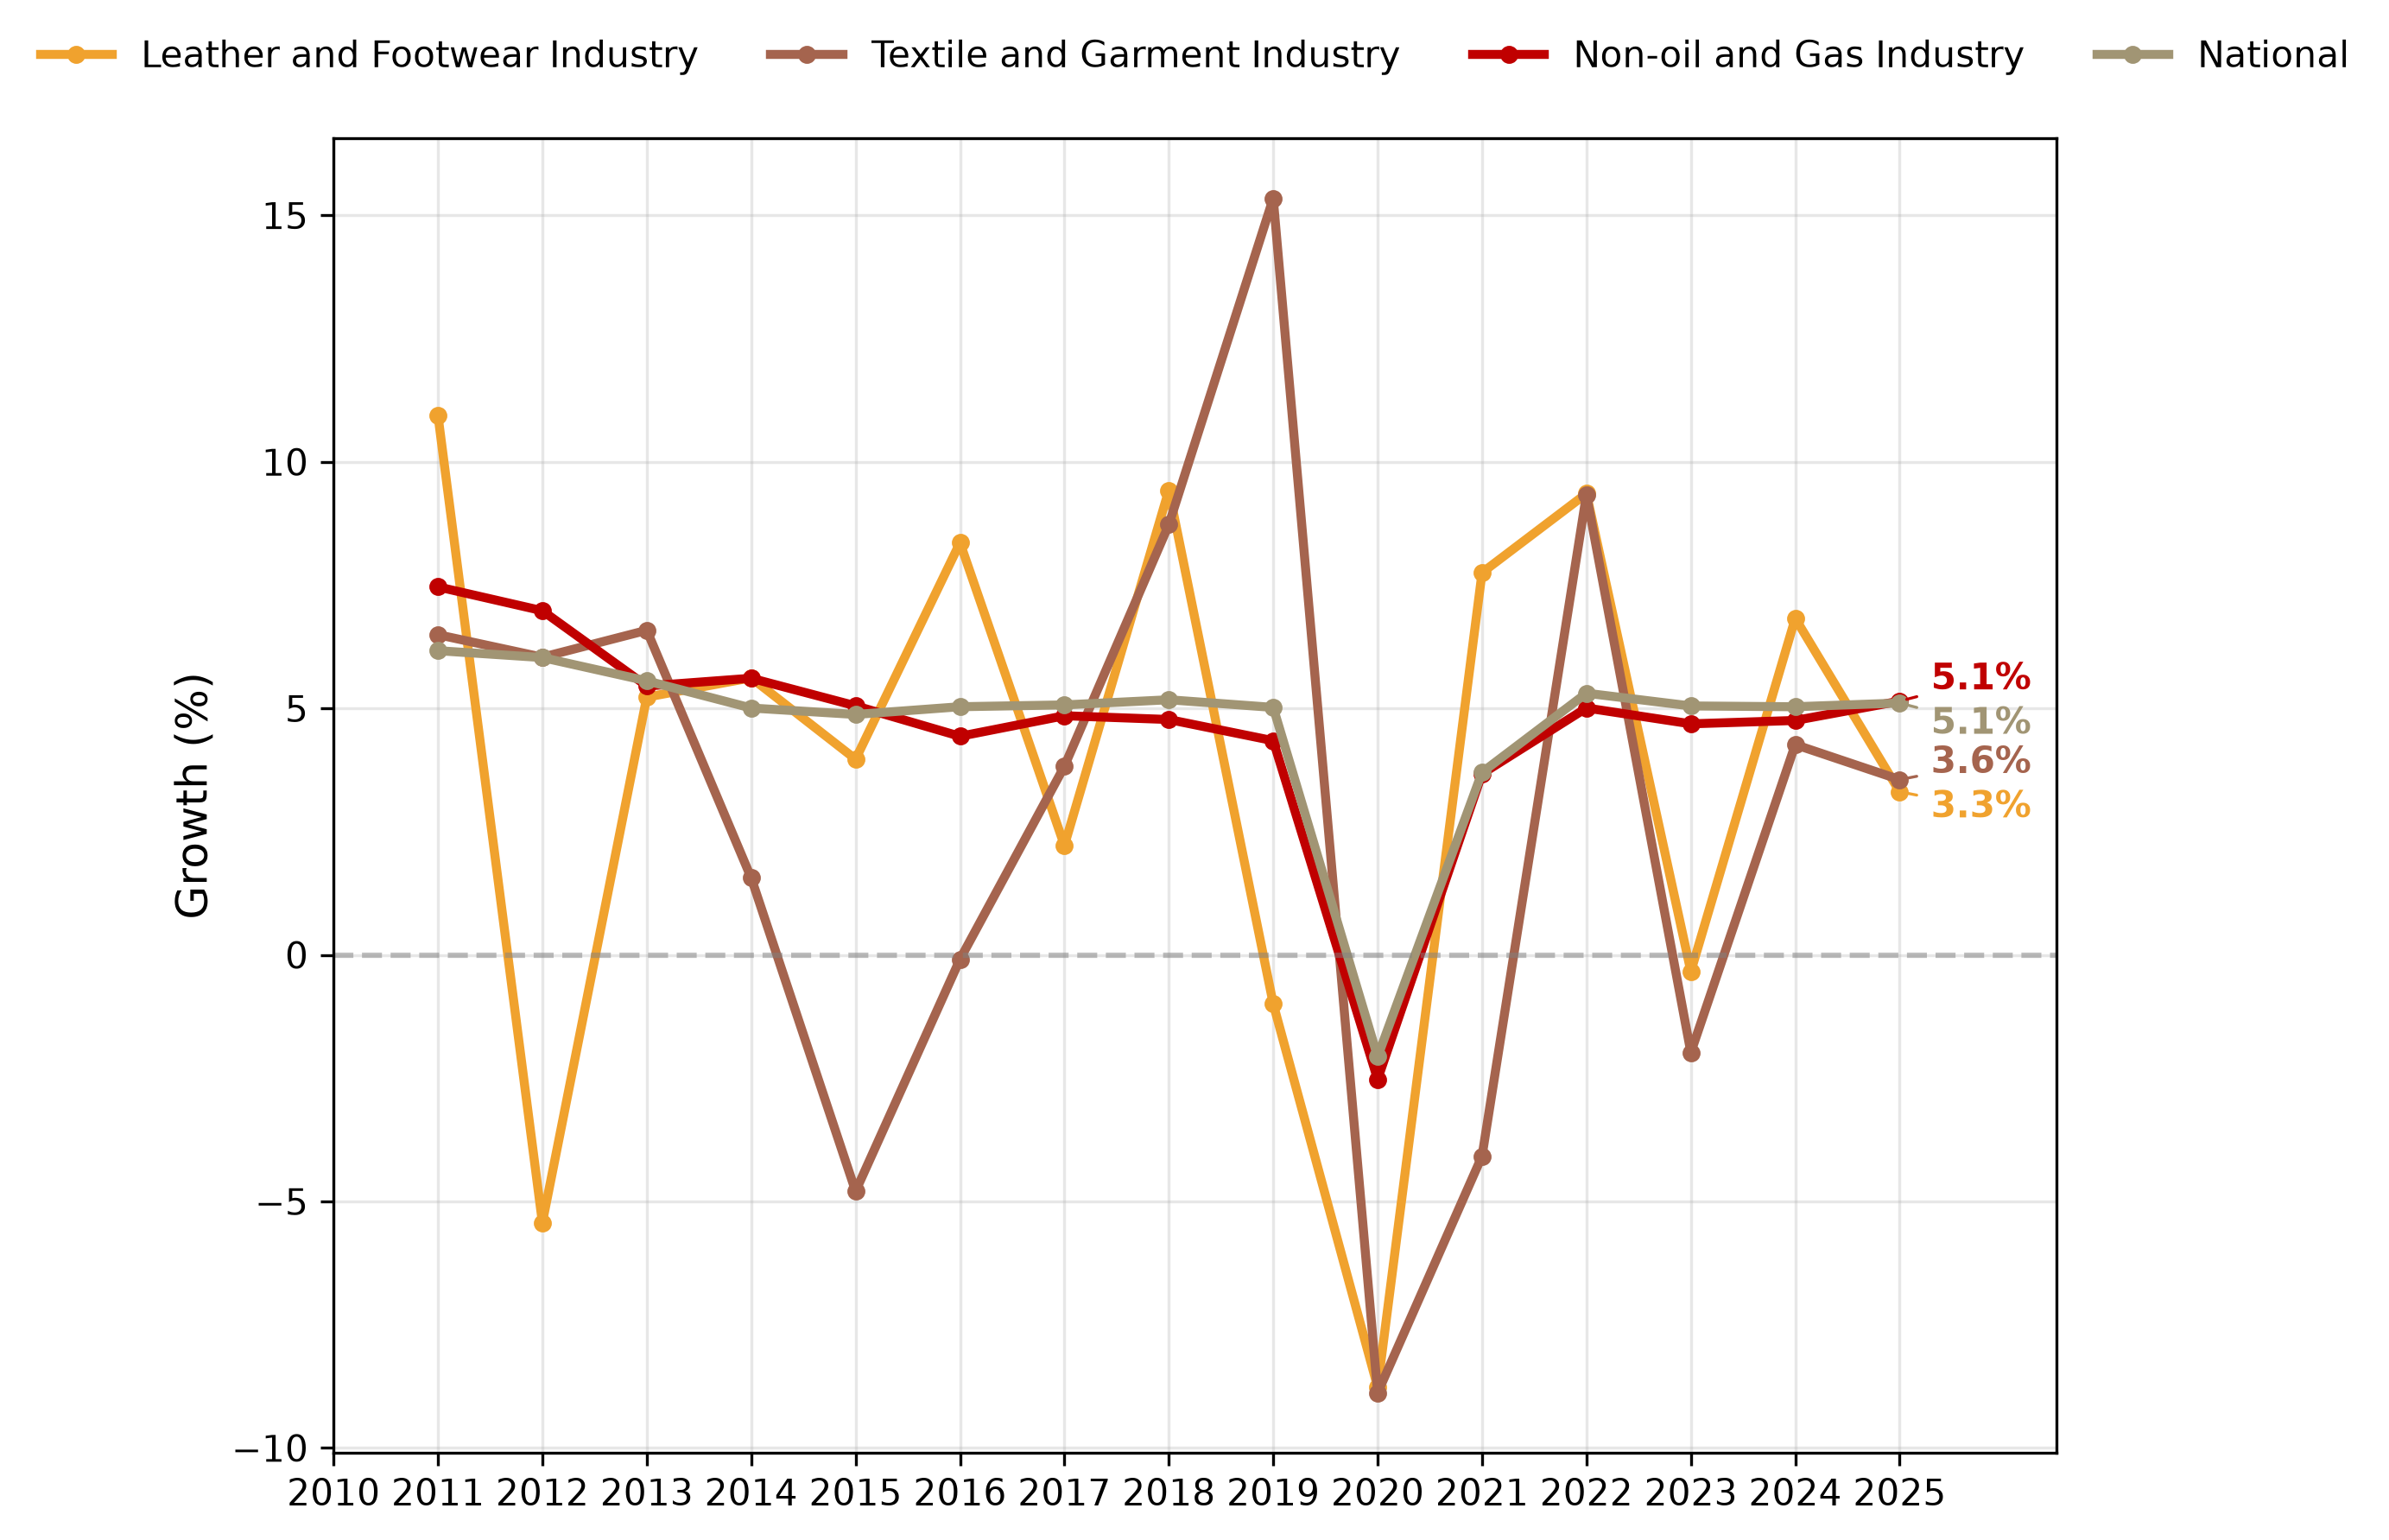
\includegraphics[width=0.85\linewidth,height=\textheight,keepaspectratio]{fig/gdp_growth.png}

}

\caption{\label{fig-growth}Growth trends in the textile, footwear and
manufacturing sectors, 2010--2025. Source: BPS.}

\end{figure}%

As Figure~\ref{fig-recovery} demonstrates, four years after the onset of
the pandemic, neither industry has fully returned to its pre-COVID
growth. The figure presents constant-price GDP for the textile \&
garment and the footwear industries. The solid, orange line represents
actual GDP data, while the dashed line indicates the pre-COVID trend
estimated using the HP filter method (Hodrick and Prescott 1997; Razzak
1997). However, the recovery path of both industries, particularly the
footwear industry, remains encouraging.

\begin{figure}[htbp!]

\centering{

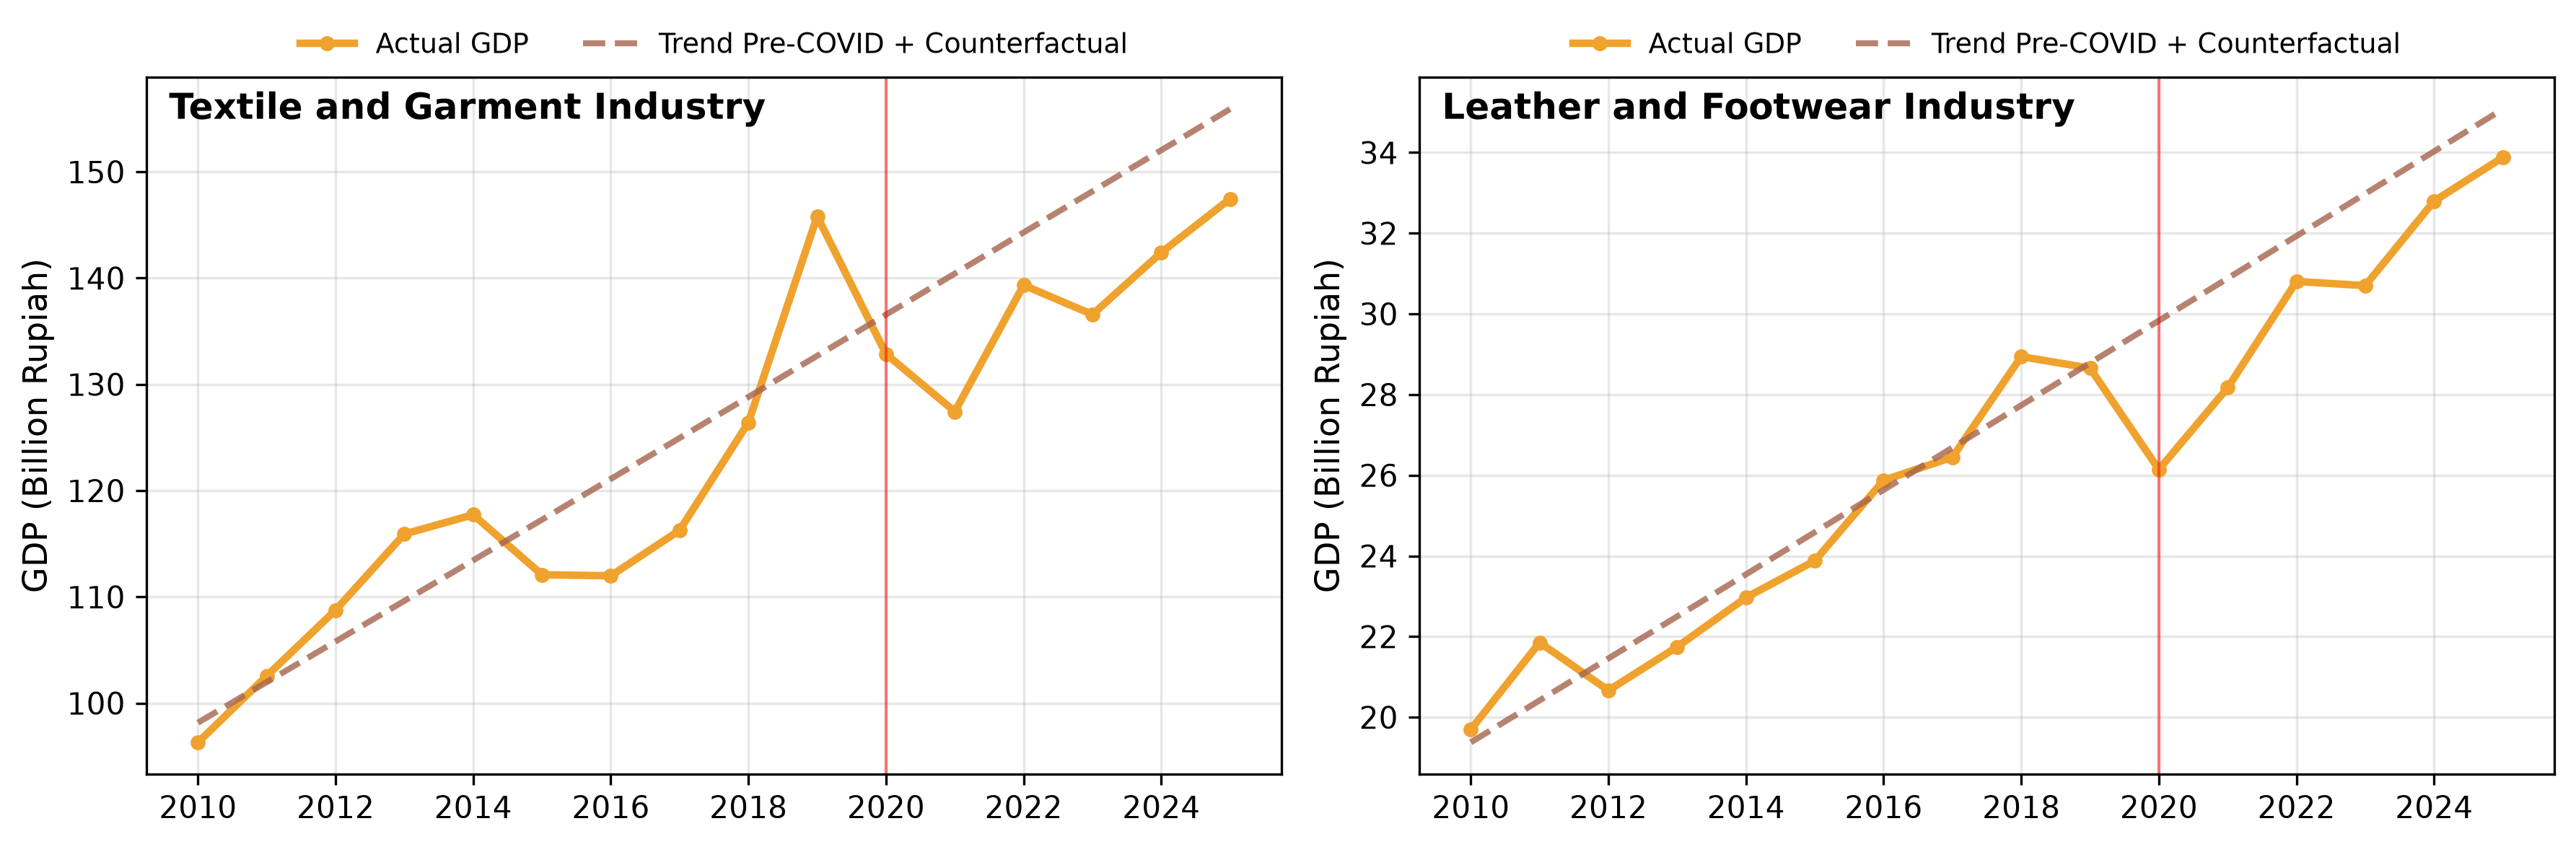
\includegraphics[width=1\linewidth,height=\textheight,keepaspectratio]{fig/gdp_covid_disruption.png}

}

\caption{\label{fig-recovery}Post-pandemic recovery projection of the
textile and footwear industries relative to pre-COVID trends. Source:
BPS, accessed through CEIC.}

\end{figure}%

Direct investment in both industries has increased substantially since
the COVID-19 pandemic, reaching their highest levels during 2021--2025
(Figure~\ref{fig-investment}). However, the two industries exhibit
markedly different investment structures. The textile and garment
industry draws from a relatively broader investment base, with domestic
investors accounting for between 19 and 61 percent of total realized
investment during 2010--2025. In contrast, the footwear industry remains
heavily dependent on foreign direct investment (FDI), with foreign
investors consistently contributing around 90 percent or more of total
investment throughout most of the period.

\begin{figure}[htbp!]

\centering{

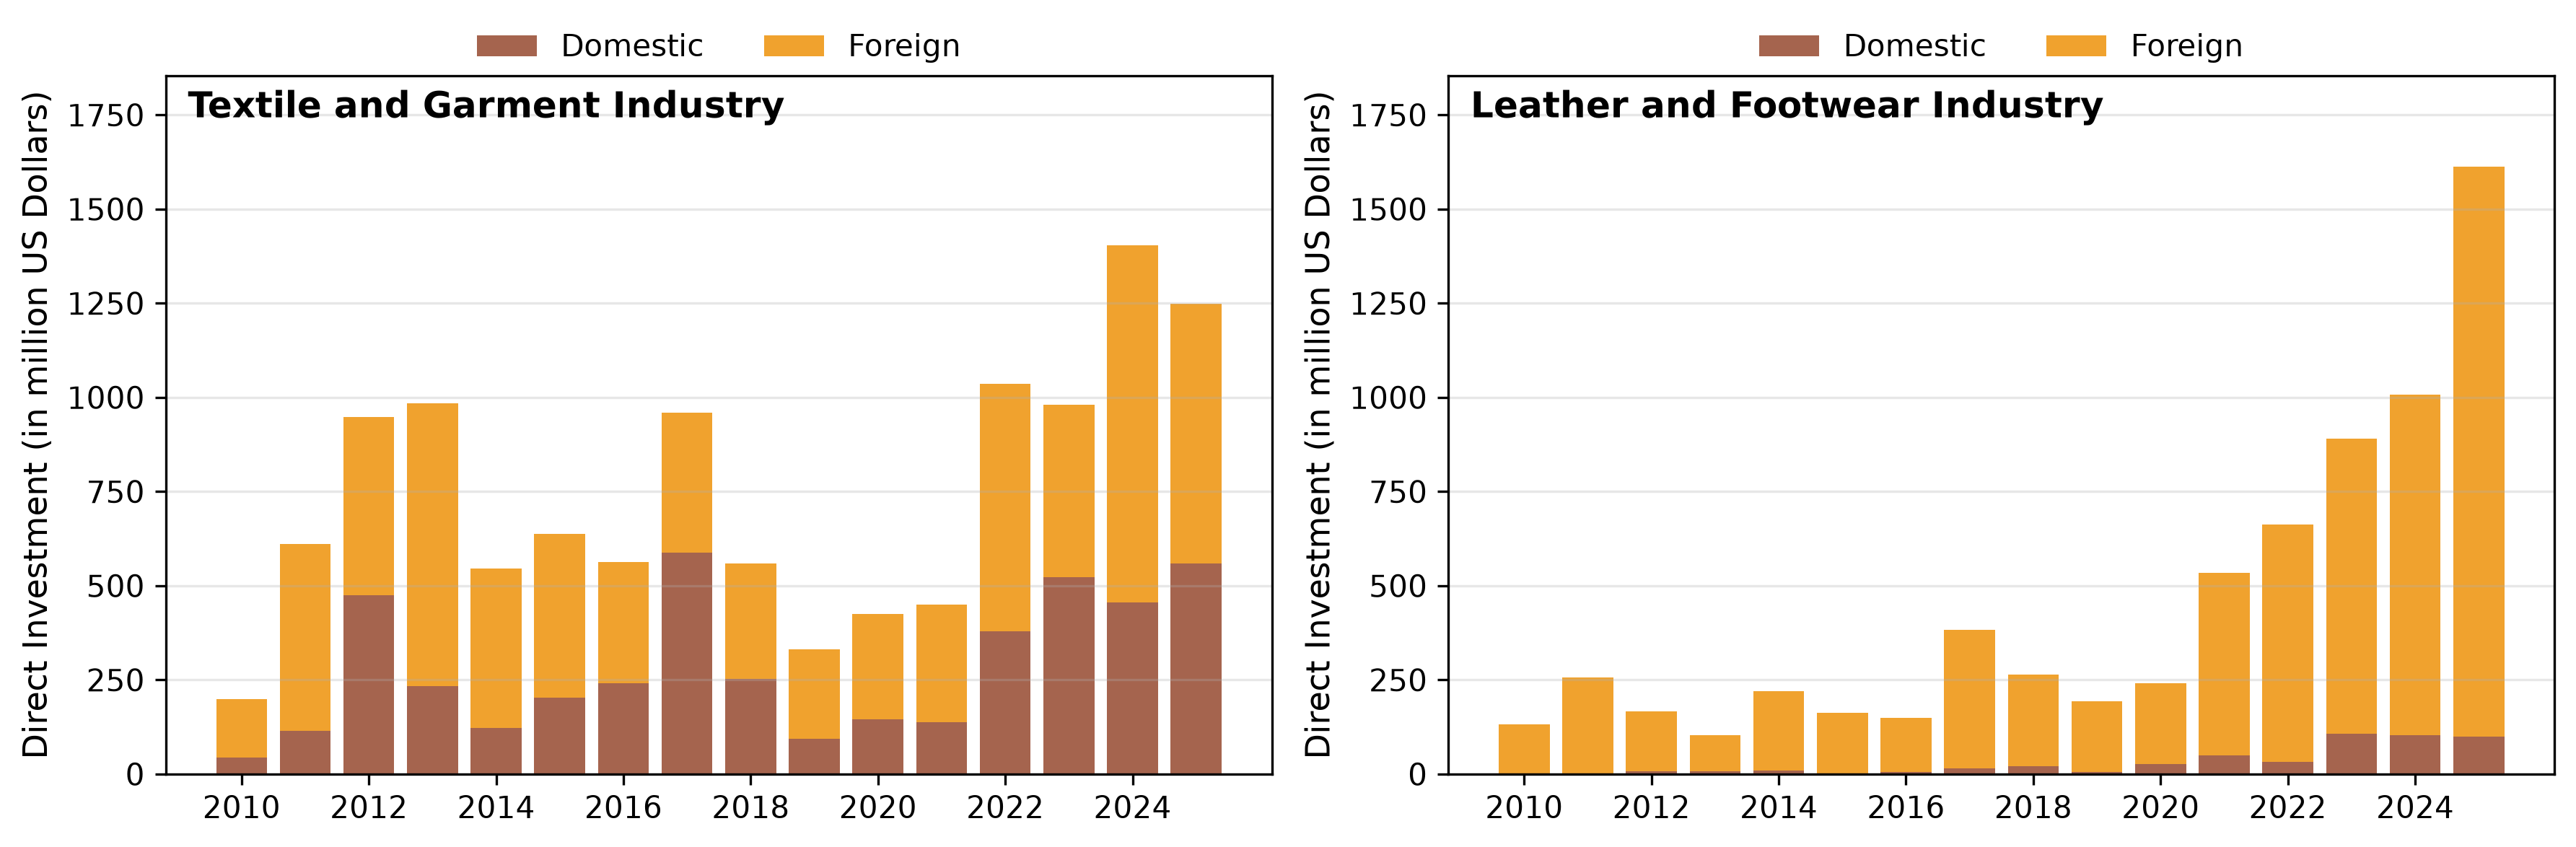
\includegraphics[width=1\linewidth,height=\textheight,keepaspectratio]{fig/investment_comparison.png}

}

\caption{\label{fig-investment}Foreign and domestic direct investment in
the textile and footwear industries, 2010--2025. Source: BPS, accessed
through CEIC.}

\end{figure}%

Investment growth has been particularly pronounced in the footwear
industry. Between 2020 and 2025, total realized investment increased
from approximately USD 241 million to more than USD 1.6 billion. Over
the same period, investment in the textile and garment industry rose
from around USD 424 million to USD 1.25 billion. As a result, by 2025
the footwear industry attracted higher levels of investment than the
textile and garment industry despite being considerably smaller in terms
of output. The predominance of foreign investment in the footwear
industry is consistent with its strong participation in export-oriented
production networks, while the textile and garment industry continues to
benefit from a more diversified mix of domestic and foreign investment.

These industries' importance is also reflected in their export
performance. In 2025, Indonesia's textile and garment industry recorded
export values of USD 11.98 billion and generated a trade surplus of USD
2.81 billion. Export values declined slightly by 0.6 percent (yoy),
compared with growth of 3.1 percent in 2024.

In contrast, the footwear industry continued to record strong export
performance. Footwear exports reached USD 7.98 billion in 2025,
increasing by 9.54 percent (yoy), compared with growth of 13.13 percent
in 2024. With imports amounting to approximately USD 1.32 billion, the
industry maintained a substantial trade surplus. These figures
underscore the continued importance of both industries as sources of
export earnings, while highlighting the stronger export momentum
currently observed in the footwear industry.

International trade plays a particularly important role in both the
textile and footwear industries. Using the Asian Development Bank's
Multi-Regional Input-Output (MRIO) Tables (Asian Development Bank 2025),
it can be estimated that approximately 41.88 percent of output from the
textile industry is ultimately allocated to export markets, while the
corresponding figure for the footwear industry reaches 92.81 percent.
Imported inputs also remain a critical component of production. Based on
estimates derived from the same MRIO framework, the value of
foreign-sourced goods and services accounts for approximately 72.88
percent of total intermediate inputs used in the textile industry and
84.23 percent in the footwear industry. These figures highlight the
extent to which both industries are integrated into regional and global
production networks, both as exporters and as users of internationally
sourced inputs.

The United States and the European Union remain the two most important
markets for global textile and footwear finished goods. Together, they
accounted for approximately 64.2 percent of global imports of products
under HS Chapters 61--64 in 2025, which mainly consist of apparel,
made-up textile articles, and footwear (Figure~\ref{fig-globalimport}).
The European Union is the world's largest importer of these products,
accounting for 47.1 percent of total global imports, followed by the
United States at 17.1 percent.

\begin{figure}[htbp!]

\centering{

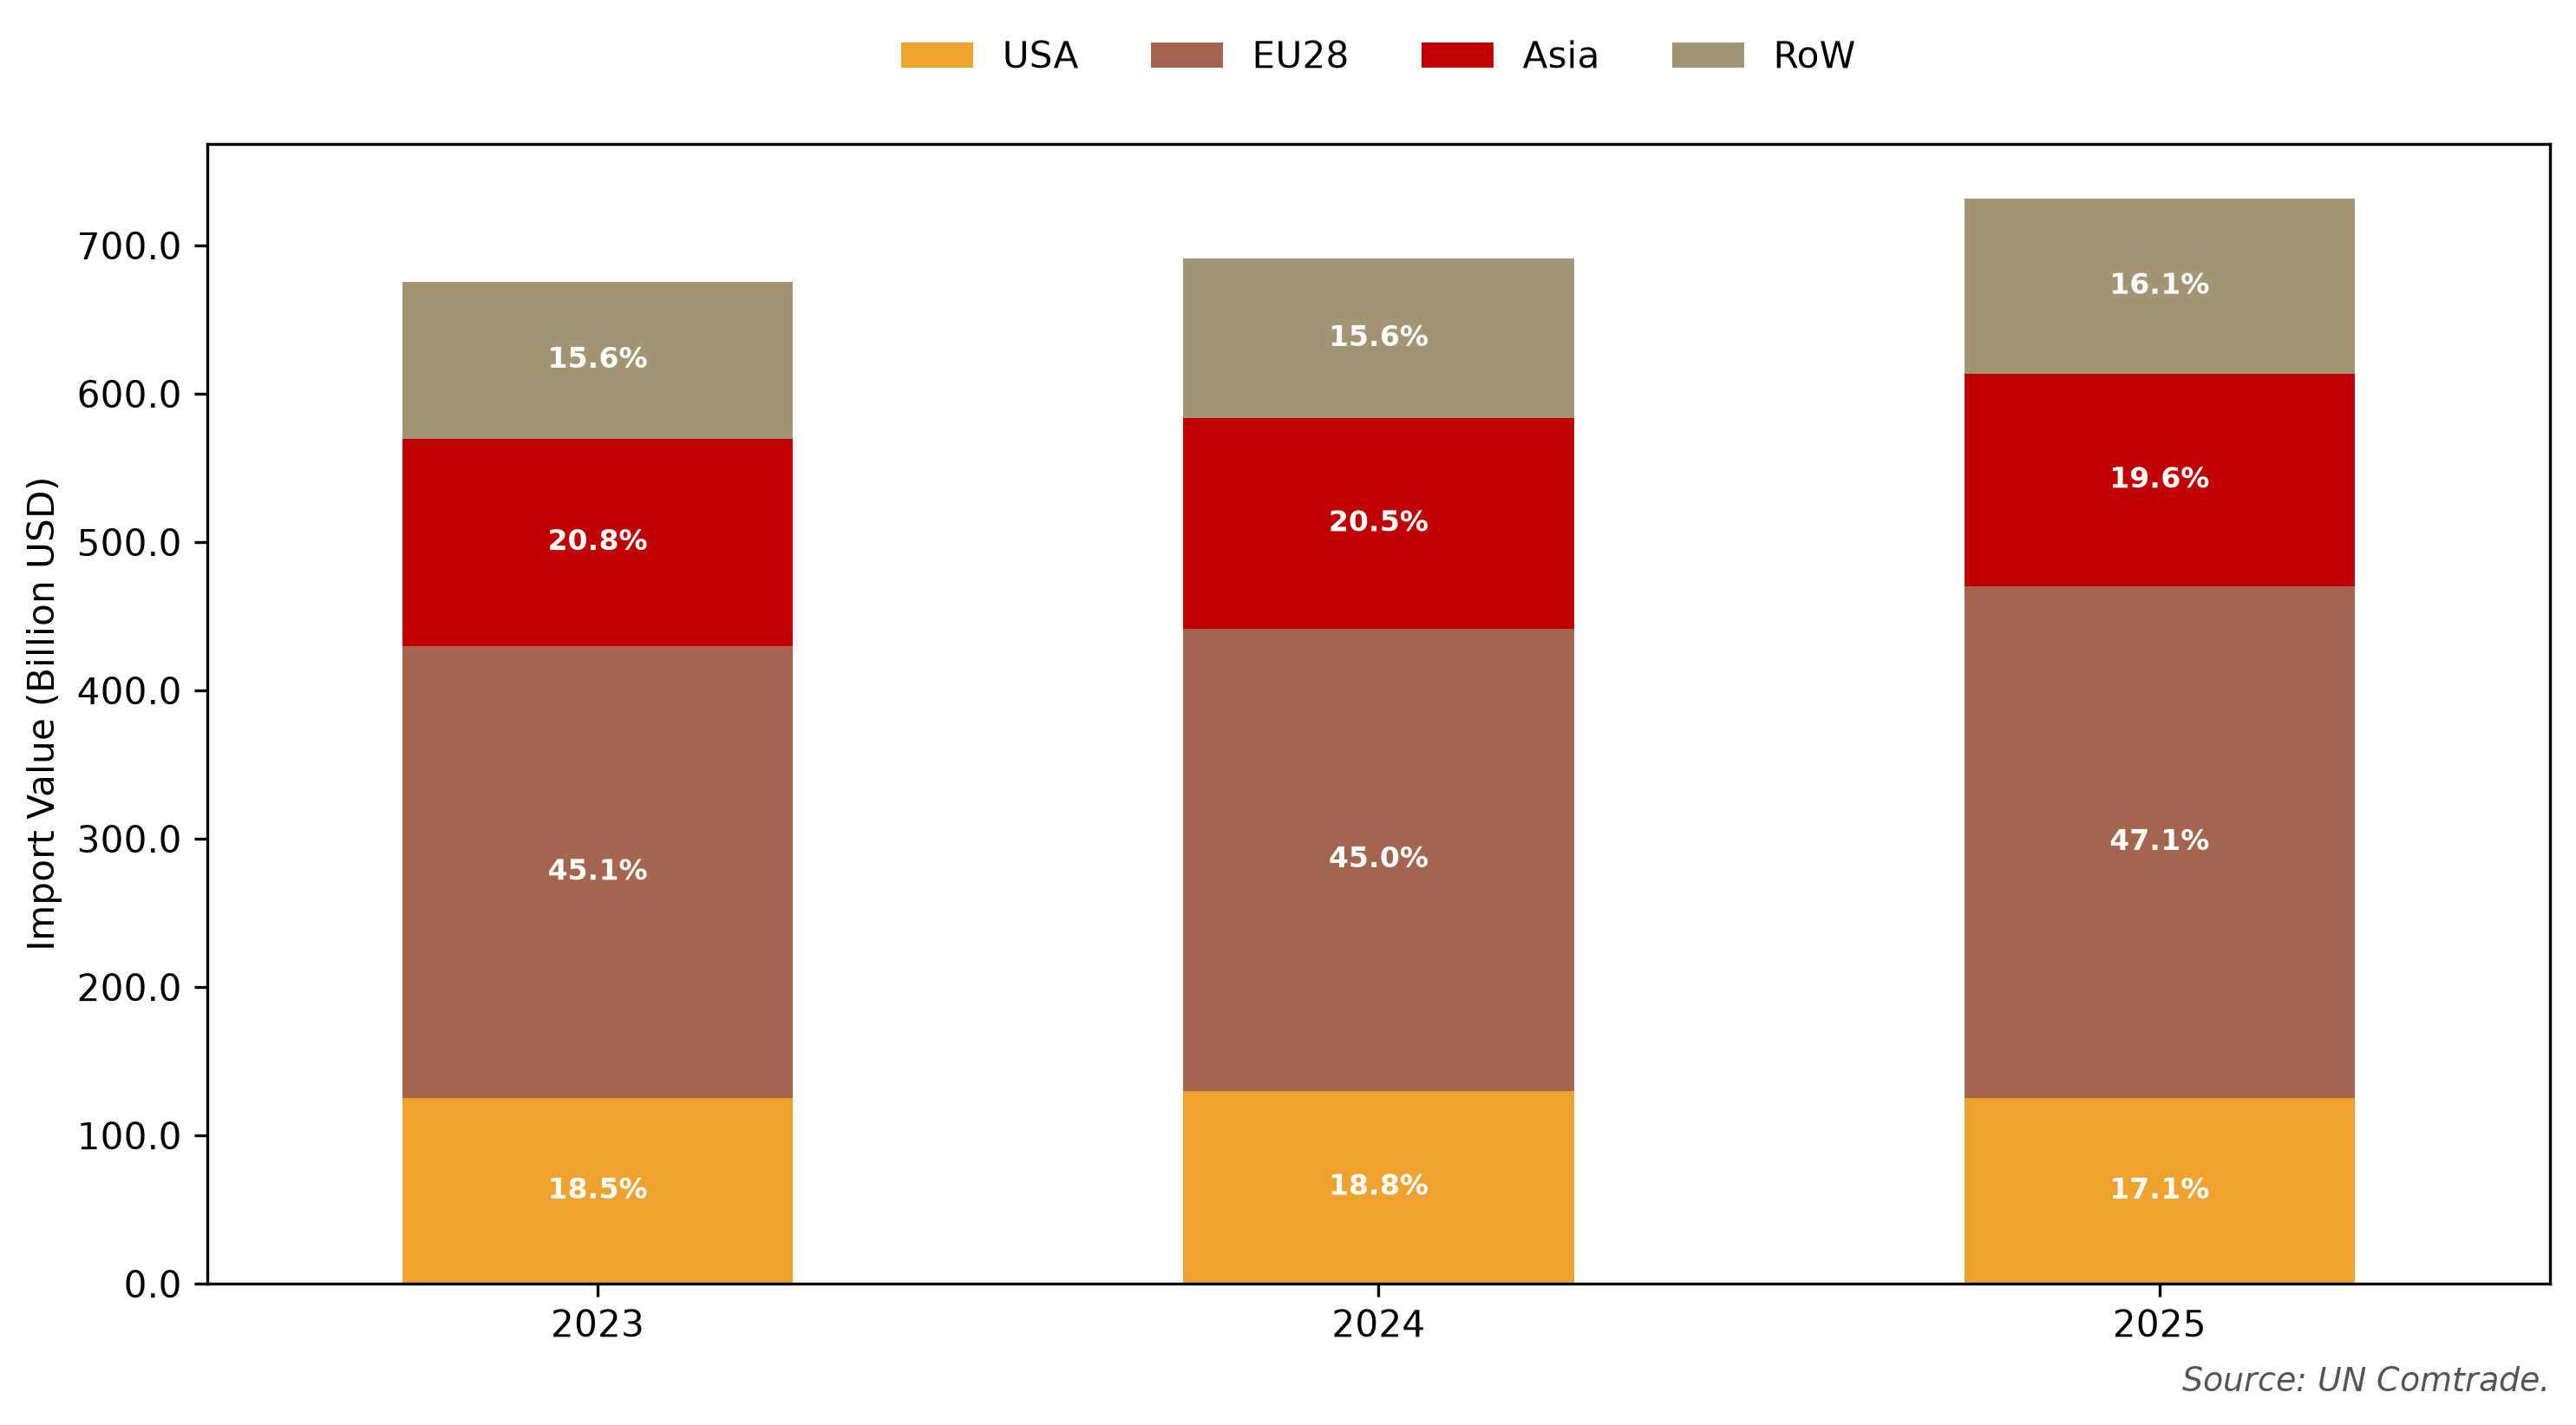
\includegraphics[width=0.85\linewidth,height=\textheight,keepaspectratio]{fig/fig1.png}

}

\caption{\label{fig-globalimport}Global import market for garments and
footwear by region, 2023--2025 (USA, EU, Asia and Rest of World (RoW)).
The y-axis shows total import value in billion USD; labels show each
region's share of global imports. Source: UN Comtrade.}

\end{figure}%

Beyond its role as a major export market, the European Union also plays
an important role in shaping global production standards through
regulatory initiatives such as the Ecodesign for Sustainable Products
Regulation (ESPR) (European Commission 2024; Yan 2025). Consequently,
sustainability and traceability requirements are becoming increasingly
important for Indonesian textile and footwear exporters seeking access
to the European market.

Table~\ref{tbl-shares} illustrates how competition in these export
markets has evolved over the past decade. Between 2015 and 2024, China's
share of textile and footwear imports declined substantially in both the
United States and the European Union. In the United States, China's
market share fell from 44.00\% to 29.22\%, while in the European Union,
it declined from 39.09\% to 30.70\%. The largest beneficiaries of this
shift were Vietnam and Bangladesh, with both countries experiencing
notable gains in market share. Indonesia recorded a modest increase in
the United States and a slight decline in the European Union. These
trends suggest that while opportunities exist for Indonesia to capture a
larger share of global demand, regional producers have generally been
more successful in expanding their market shares.

\begin{longtable}[]{@{}
  >{\raggedright\arraybackslash}p{(\linewidth - 12\tabcolsep) * \real{0.1304}}
  >{\raggedleft\arraybackslash}p{(\linewidth - 12\tabcolsep) * \real{0.1304}}
  >{\raggedleft\arraybackslash}p{(\linewidth - 12\tabcolsep) * \real{0.1304}}
  >{\raggedleft\arraybackslash}p{(\linewidth - 12\tabcolsep) * \real{0.1739}}
  >{\raggedleft\arraybackslash}p{(\linewidth - 12\tabcolsep) * \real{0.1304}}
  >{\raggedleft\arraybackslash}p{(\linewidth - 12\tabcolsep) * \real{0.1304}}
  >{\raggedleft\arraybackslash}p{(\linewidth - 12\tabcolsep) * \real{0.1739}}@{}}
\caption{Changes in U.S. and EU export market shares (percent),
2015--2024. Source: UN COMTRADE, author's
calculations.}\label{tbl-shares}\tabularnewline
\toprule\noalign{}
\begin{minipage}[b]{\linewidth}\raggedright
Partner
\end{minipage} & \begin{minipage}[b]{\linewidth}\raggedleft
US 2015
\end{minipage} & \begin{minipage}[b]{\linewidth}\raggedleft
US 2024
\end{minipage} & \begin{minipage}[b]{\linewidth}\raggedleft
US ∆ (ppt)
\end{minipage} & \begin{minipage}[b]{\linewidth}\raggedleft
EU 2015
\end{minipage} & \begin{minipage}[b]{\linewidth}\raggedleft
EU 2024
\end{minipage} & \begin{minipage}[b]{\linewidth}\raggedleft
EU ∆ (ppt)
\end{minipage} \\
\midrule\noalign{}
\endfirsthead
\toprule\noalign{}
\begin{minipage}[b]{\linewidth}\raggedright
Partner
\end{minipage} & \begin{minipage}[b]{\linewidth}\raggedleft
US 2015
\end{minipage} & \begin{minipage}[b]{\linewidth}\raggedleft
US 2024
\end{minipage} & \begin{minipage}[b]{\linewidth}\raggedleft
US ∆ (ppt)
\end{minipage} & \begin{minipage}[b]{\linewidth}\raggedleft
EU 2015
\end{minipage} & \begin{minipage}[b]{\linewidth}\raggedleft
EU 2024
\end{minipage} & \begin{minipage}[b]{\linewidth}\raggedleft
EU ∆ (ppt)
\end{minipage} \\
\midrule\noalign{}
\endhead
\bottomrule\noalign{}
\endlastfoot
China & 44.00 & 29.22 & -14.78 & 39.09 & 30.70 & -8.39 \\
Vietnam & 11.80 & 19.16 & 7.36 & 5.95 & 8.64 & 2.68 \\
India & 5.14 & 6.52 & 1.38 & 6.89 & 5.37 & -1.53 \\
Bangladesh & 4.37 & 6.03 & 1.66 & 13.12 & 16.07 & 2.95 \\
Indonesia & 5.04 & 5.46 & 0.42 & 2.66 & 2.15 & -0.52 \\
Mexico & 3.84 & 3.71 & -0.13 & 0.10 & 0.10 & 0.00 \\
Pakistan & 2.24 & 3.01 & 0.76 & 3.46 & 4.77 & 1.31 \\
Türkiye & 0.55 & 0.95 & 0.41 & 9.73 & 9.05 & -0.67 \\
\end{longtable}

It is important to note that overall, Indonesia remains relatively
competitive on several cost components, particularly in energy and water
costs. Table~\ref{tbl-costs} compares key production-cost indicators
across major textile and footwear producing countries. Wage levels in
Indonesia also remain below those in China and are broadly comparable to
those in India. Indonesia occupies a relatively competitive position as
a manufacturing base, although its advantages are not uniform across all
cost components. Indonesia's relatively modest gains in export market
share therefore cannot be explained by production costs alone. Other
factors such as supply chain integration, technology adoption, product
quality and compliance with evolving market requirements, are also
likely to play an important role in shaping competitiveness.

\begin{longtable}[]{@{}
  >{\raggedright\arraybackslash}p{(\linewidth - 10\tabcolsep) * \real{0.2857}}
  >{\raggedleft\arraybackslash}p{(\linewidth - 10\tabcolsep) * \real{0.1429}}
  >{\raggedleft\arraybackslash}p{(\linewidth - 10\tabcolsep) * \real{0.1429}}
  >{\raggedleft\arraybackslash}p{(\linewidth - 10\tabcolsep) * \real{0.1190}}
  >{\raggedleft\arraybackslash}p{(\linewidth - 10\tabcolsep) * \real{0.1905}}
  >{\raggedleft\arraybackslash}p{(\linewidth - 10\tabcolsep) * \real{0.1190}}@{}}
\caption{Comparison of production costs across Indonesia, Vietnam,
Bangladesh, Pakistan, India and China (USD and US¢). Source: Gherzi
database, WTO and ADB, accessed through Ramadhan (2025). * There is an
interest rate incentive for capital investment and technological
modernization.}\label{tbl-costs}\tabularnewline
\toprule\noalign{}
\begin{minipage}[b]{\linewidth}\raggedright
Country
\end{minipage} & \begin{minipage}[b]{\linewidth}\raggedleft
Monthly Wage (USD)
\end{minipage} & \begin{minipage}[b]{\linewidth}\raggedleft
Electricity Tariff (US¢/kWh)
\end{minipage} & \begin{minipage}[b]{\linewidth}\raggedleft
Raw Water Cost (US¢/m³)
\end{minipage} & \begin{minipage}[b]{\linewidth}\raggedleft
Cost of Capital (\% per year)
\end{minipage} & \begin{minipage}[b]{\linewidth}\raggedleft
Building Cost (USD/m²)
\end{minipage} \\
\midrule\noalign{}
\endfirsthead
\toprule\noalign{}
\begin{minipage}[b]{\linewidth}\raggedright
Country
\end{minipage} & \begin{minipage}[b]{\linewidth}\raggedleft
Monthly Wage (USD)
\end{minipage} & \begin{minipage}[b]{\linewidth}\raggedleft
Electricity Tariff (US¢/kWh)
\end{minipage} & \begin{minipage}[b]{\linewidth}\raggedleft
Raw Water Cost (US¢/m³)
\end{minipage} & \begin{minipage}[b]{\linewidth}\raggedleft
Cost of Capital (\% per year)
\end{minipage} & \begin{minipage}[b]{\linewidth}\raggedleft
Building Cost (USD/m²)
\end{minipage} \\
\midrule\noalign{}
\endhead
\bottomrule\noalign{}
\endlastfoot
Indonesia & 220 & 8 & 15 & 10\% & 263 \\
Vietnam & 275 & 7.5 & 50 & 6.50\% & 325 \\
Bangladesh & 140 & 10 & 40 & 8\% & 252 \\
Pakistan & 125 & 15 & 11 & 21\%* & 303 \\
India & 220 & 10 & 37 & 11\%* & 200 \\
China & 600 & 12 & 18 & 4.50\% & 224 \\
\end{longtable}

\subsection{Smile Curve, Global Value Chains and Economic
Dualism}\label{smile-curve-global-value-chains-and-economic-dualism}

The textile and footwear industries are characterized by a value chain
that resembles a parabola, commonly referred to as the ``smile curve''
due to its shape, illustrated by Figure~\ref{fig-smile}. The horizontal
axis represents the production process from upstream to downstream
activities, while the vertical axis represents the value added generated
at each stage of production. In both industries, value added tends to be
concentrated at the upstream and downstream ends of the value chain
(such as activities in branding, design, marketing and post-production
services), while manufacturing activities (particularly cut-make-trim
(CMT) operations) generally generate lower value added.

\begin{figure}[htbp!]

\centering{

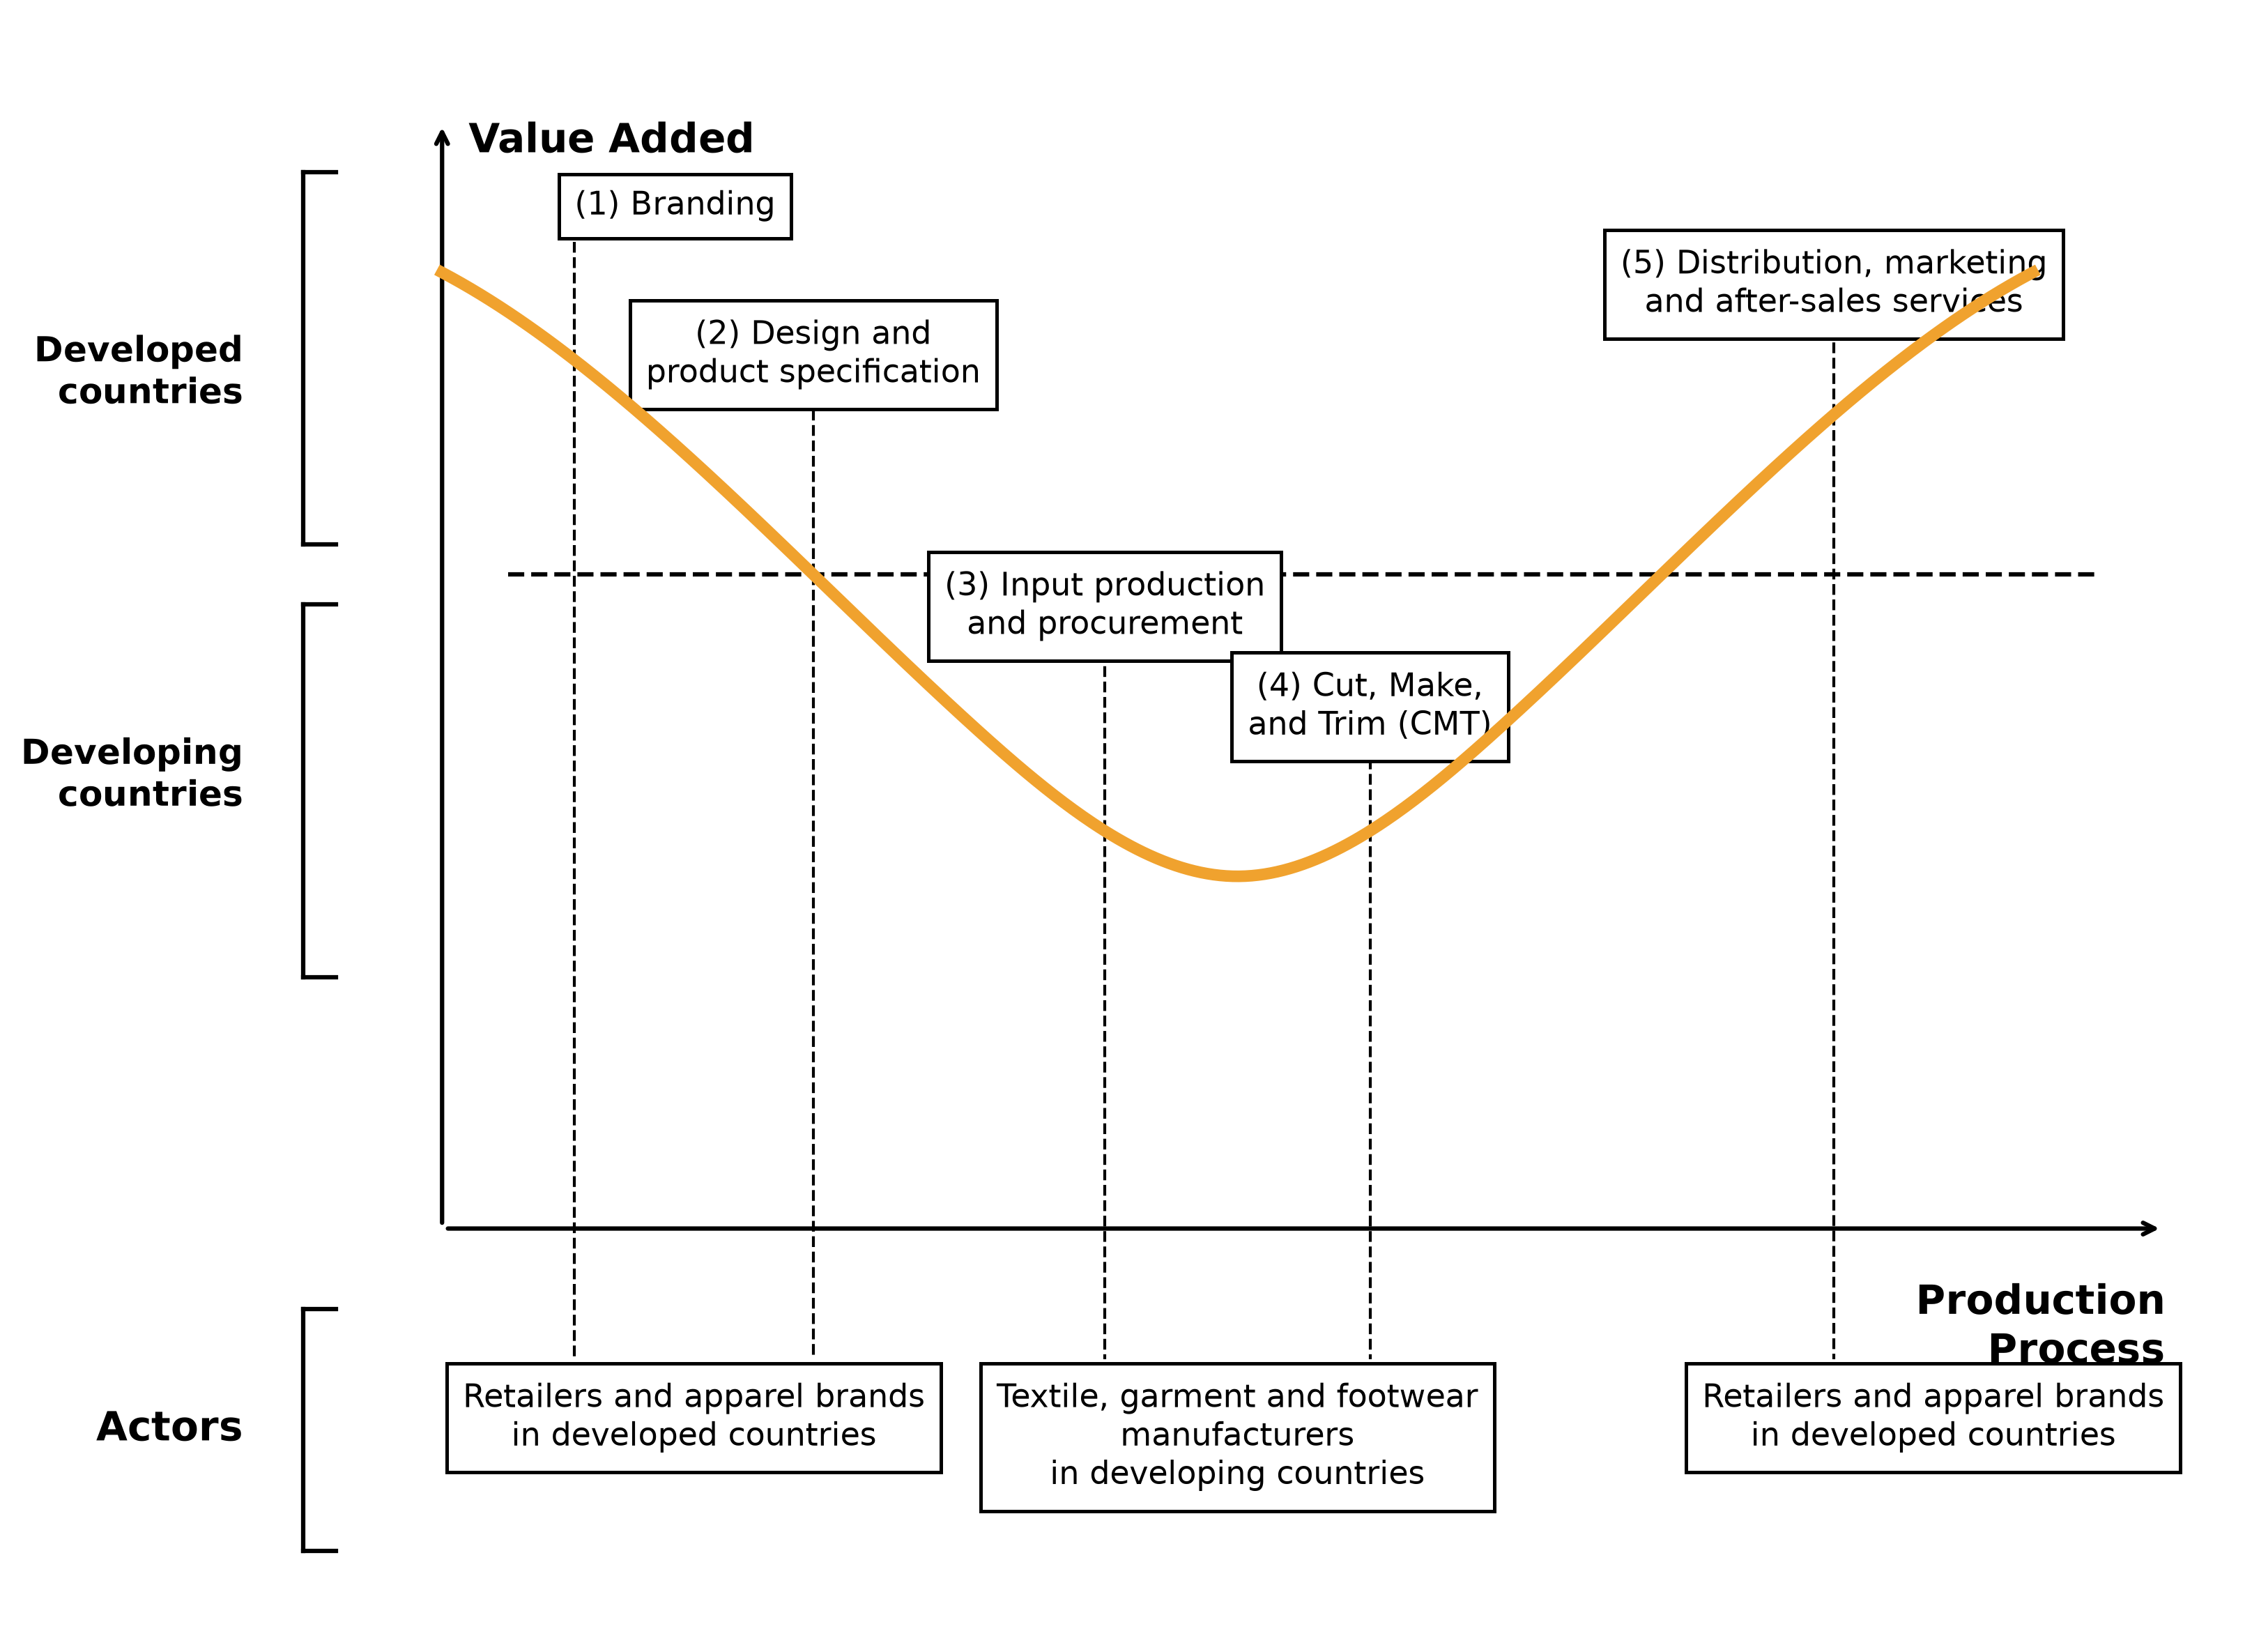
\includegraphics[width=0.9\linewidth,height=\textheight,keepaspectratio]{fig/smile_curve_english.png}

}

\caption{\label{fig-smile}Smile curve illustration in the textile and
footwear industry. Source: Goto (2023), author's calculation.}

\end{figure}%

Advances in trade, communication and logistics have enabled different
stages of production to be geographically fragmented across countries.
Higher value-added activities tend to be concentrated in economies with
stronger capabilities in design, branding, technology and specialized
services, while labor-intensive manufacturing activities are often
undertaken in countries with larger pools of general production workers.
Because production processes frequently cross national borders multiple
times before the product reaches the final consumer, this phenomenon is
commonly referred to as a Global Value Chain (GVC) (Feenstra and Taylor
2021; Gereffi and Frederick 2010; Gupta, Choirinnida, and Taufik 2022).

Many textile and footwear firms operating in Indonesia are integrated
into these GVCs. These firms typically function as contract
manufacturers to global brands such as Nike, Adidas, H\&M and Uniqlo
(often referred to as buyers or principals). The principals ultimately
retain control over product design, quality standards, sourcing
decisions, logistics and marketing, while the manufacturers primarily
provide production services. It is important to note that both raw
material and finished goods generally remain under the ownership of the
principal throughout the production process. Therefore, any of
Indonesia's export statistics will only capture the manufacturing fee,
not the embedded, higher value that comes from, for example, design and
branding.

Ultimately, Indonesia participates primarily in the manufacturing
segment of the value chain, where value added is relatively low, while
higher value activities such as branding, design and marketing remain
concentrated with the global lead firms. As a result, the export value
(measured on a Free on Board basis) primarily captures the manufacturing
stage of production undertaken in Indonesia. It does not reflect the
substantially higher retail value generated in downstream stages of the
value chain.

Given their integration into global value chains, Bonded Zones play an
important role in supporting Indonesia's export-oriented textile and
footwear industries. Under the Ministry of Finance Regulation
No.~131/2018, Bonded Zones are designated areas where imported and/or
local supplies to be processed can be stored prior to export or domestic
use. Facilities located in Bonded Zones benefit from reduced
administrative and tax-related burdens associated with importing
machinery and production inputs, thereby supporting the competitiveness
of the export-oriented manufacturers. According to Masitoh (2024), 453
of the 1455 firms receiving Bonded Zone facilities were textile and
garment firms, equivalent to 11.60\% of all textile and garment
companies in Indonesia.

Alongside these globally integrated firms, Indonesia also has a large
number of independent domestic producers that are not directly
integrated into GVCs. Unlike export-oriented contract manufacturers,
these firms typically operate under their own brands, procure their own
inputs and market their products directly to retailers and consumers.
They are highly diverse, ranging from medium-sized manufacturers
supplying domestic retail chains, to small and micro enterprises, to
artisanal producers rooted in regional craft traditions.

This group is generally oriented toward the domestic market and relies
primarily on domestic investment. In addition, many of these producers
have limited access to proprietary design capabilities or advanced
production technology and rely on imported inputs and machinery that may
not be covered by the facilitation available to Bonded Zone operators.
Their production processes tend to be less complex and are subject to
fewer compliance requirements related to the quality standards imposed
by global buyers or even the ESPR.

This has given rise to a form of economic dualism within Indonesia's
textile and footwear industries. On one side, there are large-scale,
often foreign invested firms integrated into GVCs and linked to
international buyers. On the other are smaller firms and artisans
primarily serving the domestic market. These two groups differ
significantly in terms of business models, production structures and
competitive challenges. As a result, policy interventions that are
effective for globally integrated exporters may not address and/or
capture the constraints faced by domestically oriented producers, and
vice versa. Recognizing this distinction is therefore essential for
effective policy making. Meanwhile, understanding the deeper structural
roots requires examining how Indonesia is positioned within the global
chains.

\subsection{Overview of the Textile \& Garments
Industry}\label{overview-of-the-textile-garments-industry}

Indonesia's textile industry spans the full length of the smile curve,
and consists of a vertically integrated production chain extending from
upstream raw material processing to downstream garment manufacturing and
retail activities (Figure~\ref{fig-textilechain}). Upstream segments,
including the processing of petrochemical inputs such as PTA/MEG,
polyester fiber production and yarn spinning, tend to be capital and
energy intensive. Meanwhile, production becomes more labor-intensive
moving downstream, culminating in garment manufacturing and the retail
sector. This structural distinction has direct implications for the
types of value added generated, the employment profiles supported and
the nature of competitive pressures faced at each stage.

\begin{figure}[htbp!]

\centering{

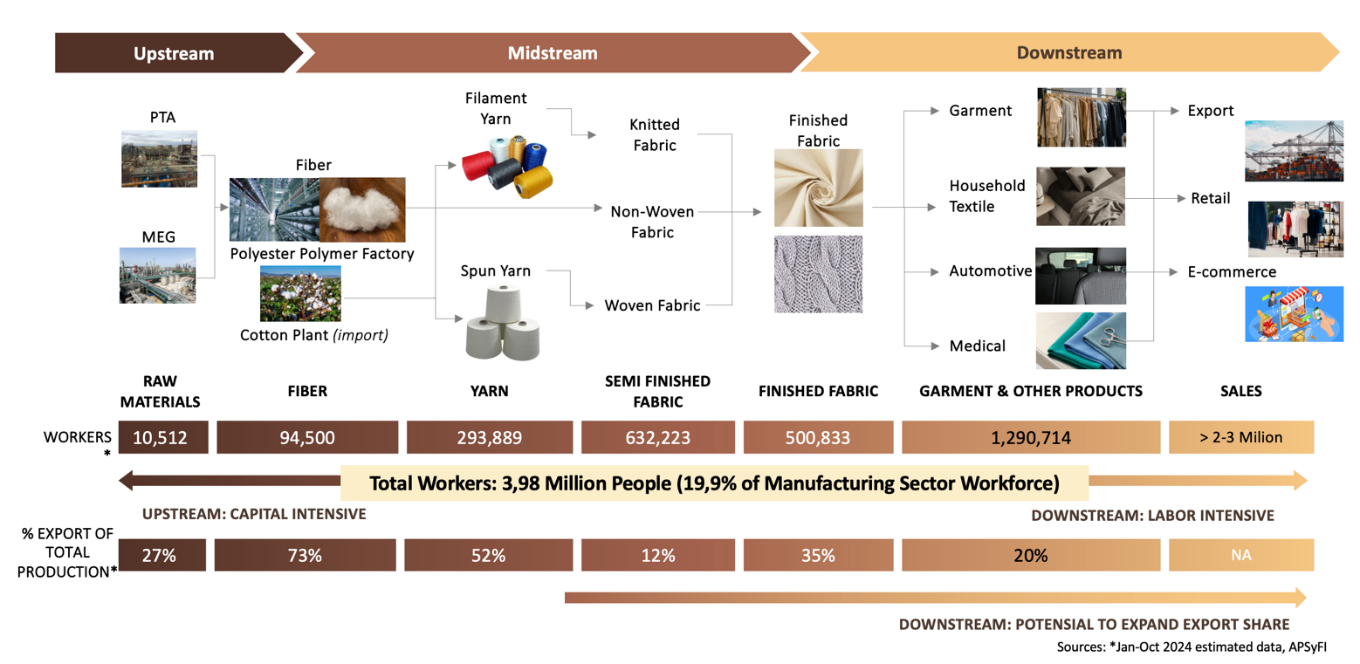
\includegraphics[width=1\linewidth,height=\textheight,keepaspectratio]{fig/textile_value_chain.png}

}

\caption{\label{fig-textilechain}Structure of the textile industry value
chain. Source: BPS, International Textile Manufacturers Federation.}

\end{figure}%

Indonesia's upstream textile segments demonstrate a relatively strong
export orientation. Fiber and yarn production export shares reach 73\%
and 52\%, respectively (Figure~\ref{fig-textilechain}). By contrast,
downstream activities such as garment manufacturing export 20.00\% of
their total production. However, employment increases along the value
chain, rising from approximately 10,000 workers in raw material
processing (PTA/MEG) to more than 1.29 million workers in garment
manufacturing.

The complementary roles performed across different segments of the value
chain underscore the textile industry's broader strategic importance.
Upstream segments contribute to export earnings and integration into
GVCs, while downstream segments serve as a major source of formal
employment and income. These differences highlight the need for
differentiated policy approaches that recognize the distinct
constraints, capabilities and opportunities facing firms across segments
of the value chain.

The geographic distribution of Indonesia's textile industry indicates
that production activity remains heavily concentrated on the island of
Java (Figure~\ref{fig-maptextile}). Of the 761 textile firms recorded,
nearly 57\% are located in West Java, serving as the primary hub of
Indonesia's textile industry, supported by the availability of labor,
supporting infrastructure, and proximity to markets and supply chains.
Central Java (18\%) and Banten (10\%) also play important roles as major
industrial clusters, while East Java (9.2\%) continues to contribute
through its concentration of medium-scale industries. Together, these
provinces form the core of Indonesia's textile manufacturing base.

\begin{figure}[htbp!]

\centering{

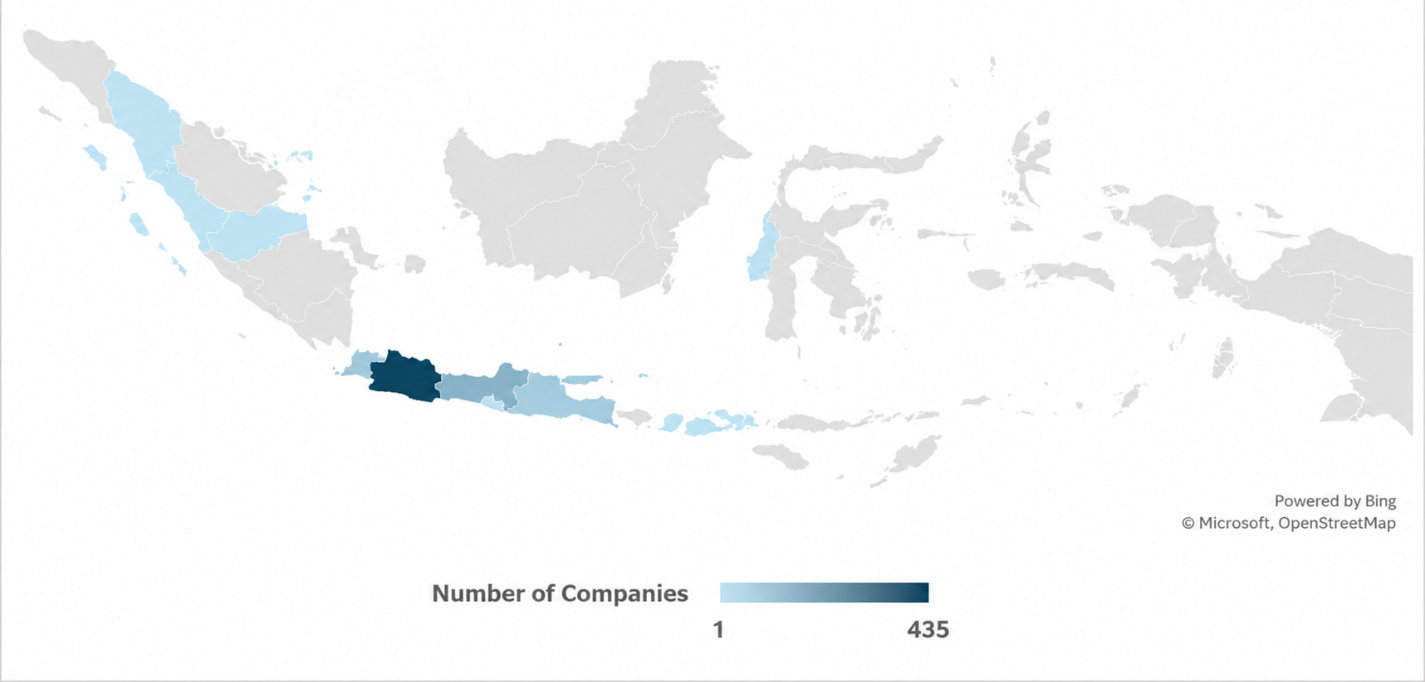
\includegraphics[width=1\linewidth,height=\textheight,keepaspectratio]{fig/map_textile.png}

}

\caption{\label{fig-maptextile}Distribution map of companies in the
textile industry. Source: BPS, author's calculation.}

\end{figure}%

Outside of Java (2.37\%), textile manufacturers are far fewer in number
and more geographically dispersed. Many of these enterprises have
emerged from local traditions such as weaving and textile handicrafts.
This illustrates the structural heterogeneity at the firm-level where
large scale, GVC-integrated manufacturers coexist alongside domestically
oriented producers, MSMEs and artisanal enterprises, each facing
distinct competitive conditions and policy needs.

\subsection{Overview of the Footwear
Industry}\label{overview-of-the-footwear-industry}

Indonesia's footwear industry is similarly characterized by a
multi-stage production process spanning raw material suppliers,
component manufacturers, footwear assembly and distribution to final
consumers (Figure~\ref{fig-footwearchain};
Figure~\ref{fig-footwearprocess}). Inputs such as leather, rubber,
textiles, synthetic materials and chemical components are transformed
into footwear parts before being assembled into finished products. While
value creation in the industry extends beyond manufacturing to
activities such as design, product development, branding, and
innovation, production activities remain the dominant segment undertaken
in Indonesia.

\begin{figure}[htbp!]

\centering{

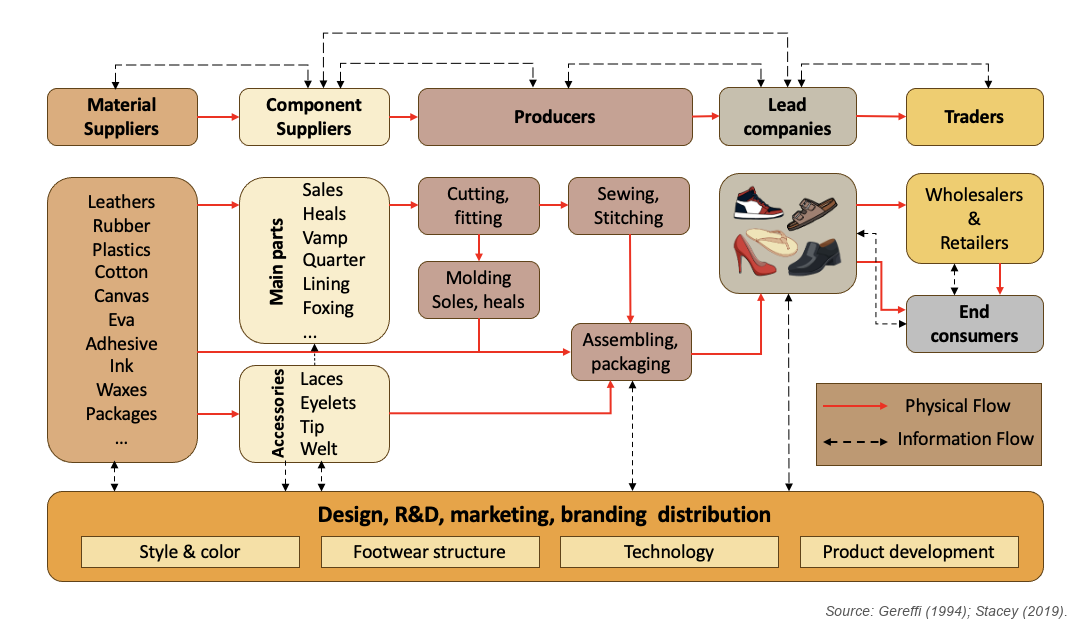
\includegraphics[width=1\linewidth,height=\textheight,keepaspectratio]{fig/footwear_supply_chain.png}

}

\caption{\label{fig-footwearchain}Footwear supply chain. Source: Gereffi
(1994); Stacey (2019).}

\end{figure}%

\begin{figure}[htbp!]

\centering{

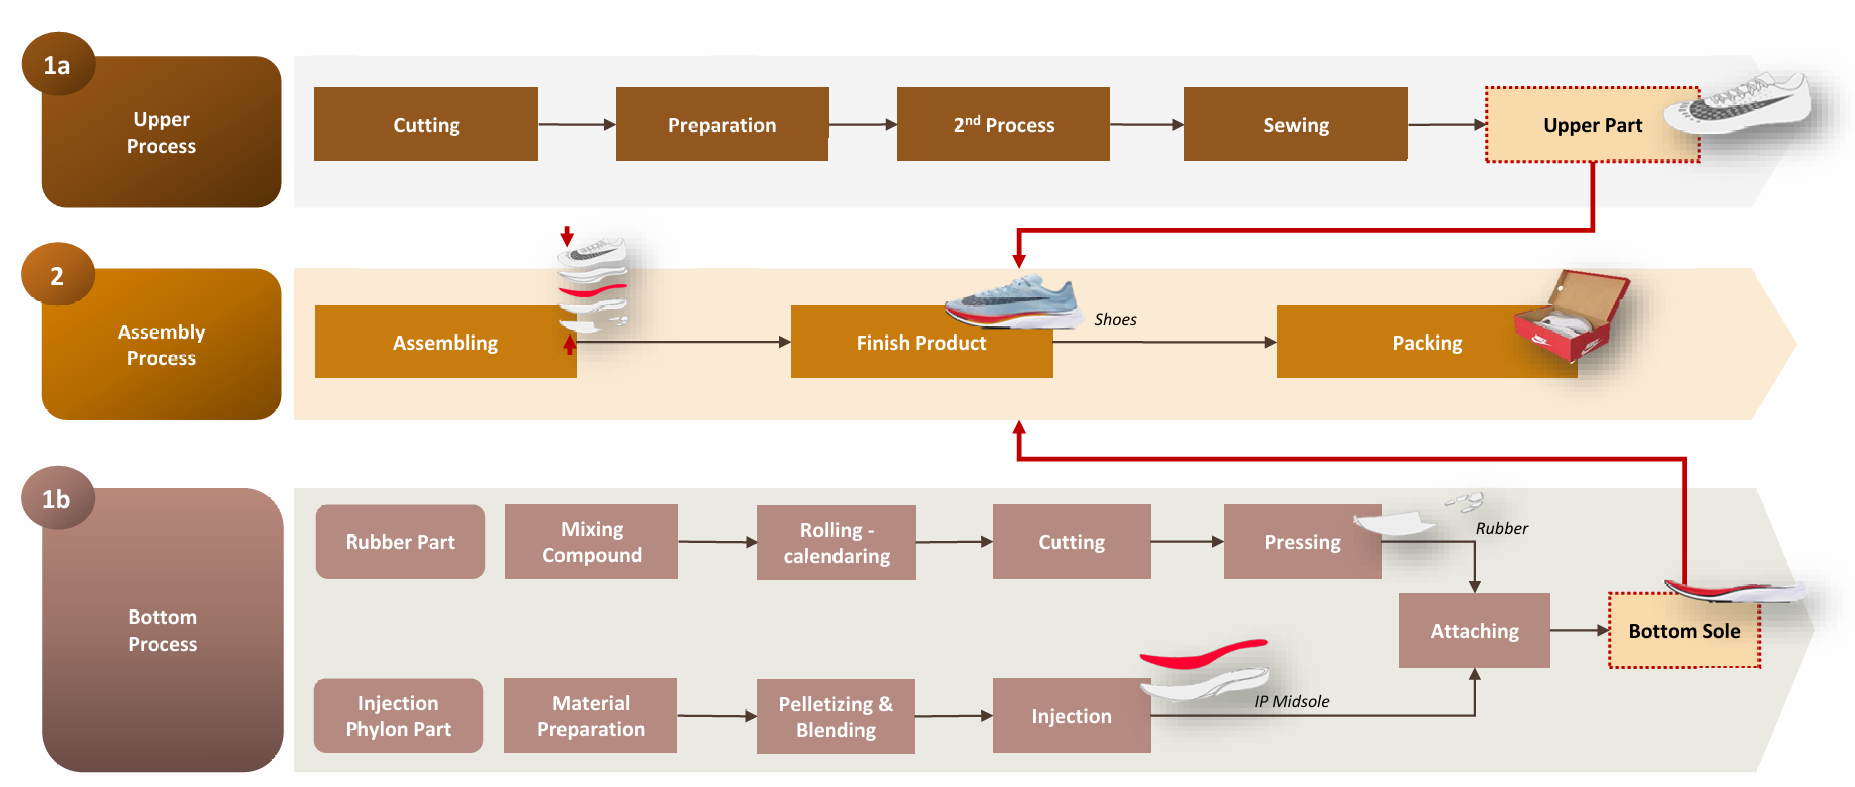
\includegraphics[width=1\linewidth,height=\textheight,keepaspectratio]{fig/footwear_production_process.png}

}

\caption{\label{fig-footwearprocess}Factory production process for the
footwear industry. Source: DEN (2025), based on site visits and
interviews with footwear manufacturers.}

\end{figure}%

Many of Indonesia's footwear manufacturers are integrated into the GVC,
supplying international brands through export-oriented production
networks. As previously mentioned, these firms typically specialize in
manufacturing activities within the value chain, while higher-value
added functions are often undertaken by global lead firms. The footwear
industry's heavy reliance on FDI (accounting for approximately 90\% of
total investment) reflects this deep integration into international
production networks.

At the same time, Indonesia's footwear industry continues to face
structural challenges in upstream segments. Dependence on imported
inputs remains high, estimated at between 60--70\% (Ministry of Industry
2024). Consistent with the smile curve framework, Indonesia's
comparative strength remains concentrated in downstream production
activities, while upstream capabilities remain relatively
underdeveloped. This represents a structural consideration for long-term
competitiveness that warrants continued attention, even as Indonesian
footwear products continue to perform well in international markets.

The footwear industry's production base is heavily concentrated on the
island of Java (Figure~\ref{fig-mapfootwear}). West Java hosts the
largest number of globally integrated footwear factories, with 42
facilities employing more than 186,000 workers across Sukabumi, Garut,
Cibogo and Karawang. Banten and Central Java are home to 29 and 13
factories, respectively, each province employing just over 112,000
workers. The concentration of production in these provinces is supported
by industrial infrastructure, access to suppliers and established export
networks.

\begin{figure}[htbp!]

\centering{

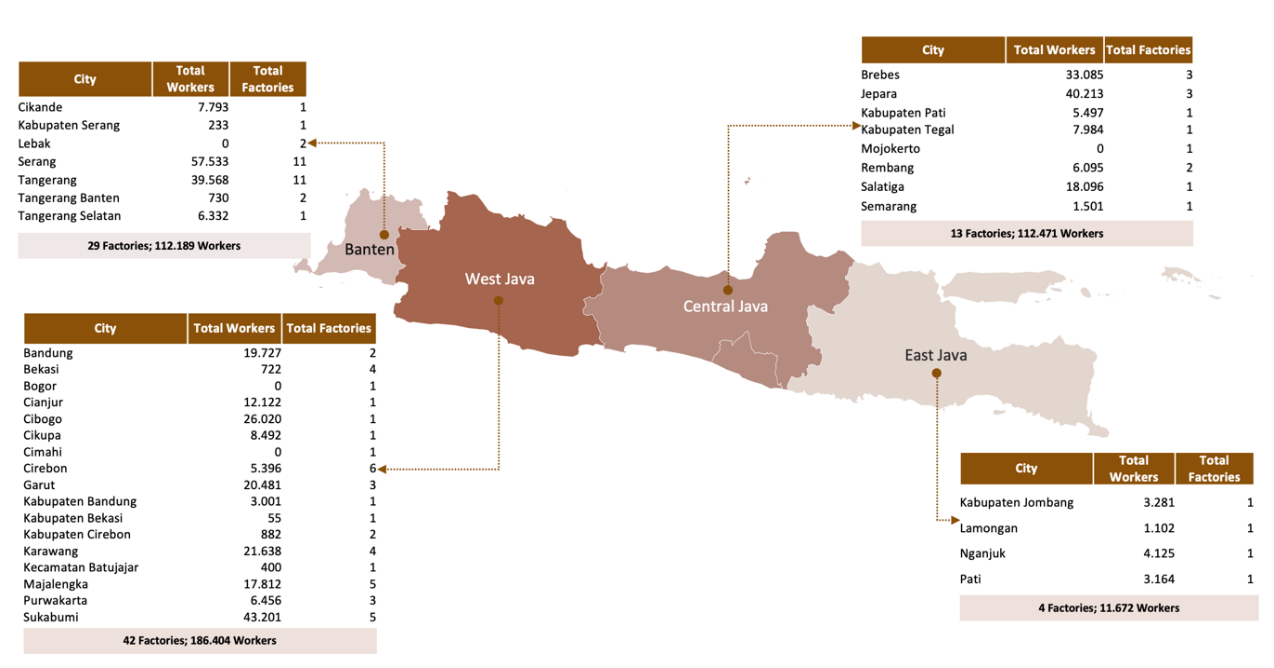
\includegraphics[width=1\linewidth,height=\textheight,keepaspectratio]{fig/map_footwear.png}

}

\caption{\label{fig-mapfootwear}Geographic distribution of footwear
factories in Java. Source: APRISINDO (2025); DEN analysis.}

\end{figure}%

Recent investment trends suggest that Central Java is emerging as an
increasingly important destination for footwear manufacturing expansion.
While West Java and Banten remain the industry's largest production
centers, relatively lower labor costs and the availability of workers
have encouraged firms to establish new facilities and expand existing
operations in Central Java. Employment in Central Java's footwear
industry is expected to increase by approximately 85,000
workers\footnote{Based on DEN interviews and authors' estimates using
  planned expansions by two major global footwear manufacturers and
  their supplier networks in Central Java (2025).} over the next one to
two years, underscoring the growing importance of the region within
Indonesia's footwear manufacturing landscape.

This highlights the extent to which developments in Java continue to
shape the performance of Indonesia's footwear industry. Given the
concentration of manufacturers on the island, efforts to strengthen
competitiveness (such as through infrastructure improvements, human
capital development and investment incentives) will depend heavily on
effective coordination between the central government and provincial
government in these key production centers.

\section{Strategic Issues in the Textile \& Garments and Footwear
Industry}\label{strategic-issues-in-the-textile-garments-and-footwear-industry}

The strategic challenges facing Indonesia's textile and footwear
industry are shaped by the sector's economic dualism and heterogeneous
industrial structure. Two implications are particularly important.
First, the existence of a relatively complete value chain does not
necessarily imply strong integration across all segments. Second,
different segments of the industry often face fundamentally different
constraints and policy needs.

Figure~\ref{fig-trade} illustrates the first implication. Although
Indonesia has developed a substantial upstream textile industry, the
country continues to simultaneously import and export significant
volumes of textile raw materials and intermediate goods. The rayon
industry provides a useful example. Indonesia is a competitive producer
of viscose-based products, yet firms in this segment remain deeply
integrated into international markets. Asia Pacific Rayon (APR), for
instance, exports 61\% of its Viscose Staple Fibre (VSF) production and
71\% of its Viscose Yarn output, while Indonesia continues to import
rayon and yarn products from abroad (Asia Pacific Rayon 2024).

\begin{figure}[htbp!]

\centering{

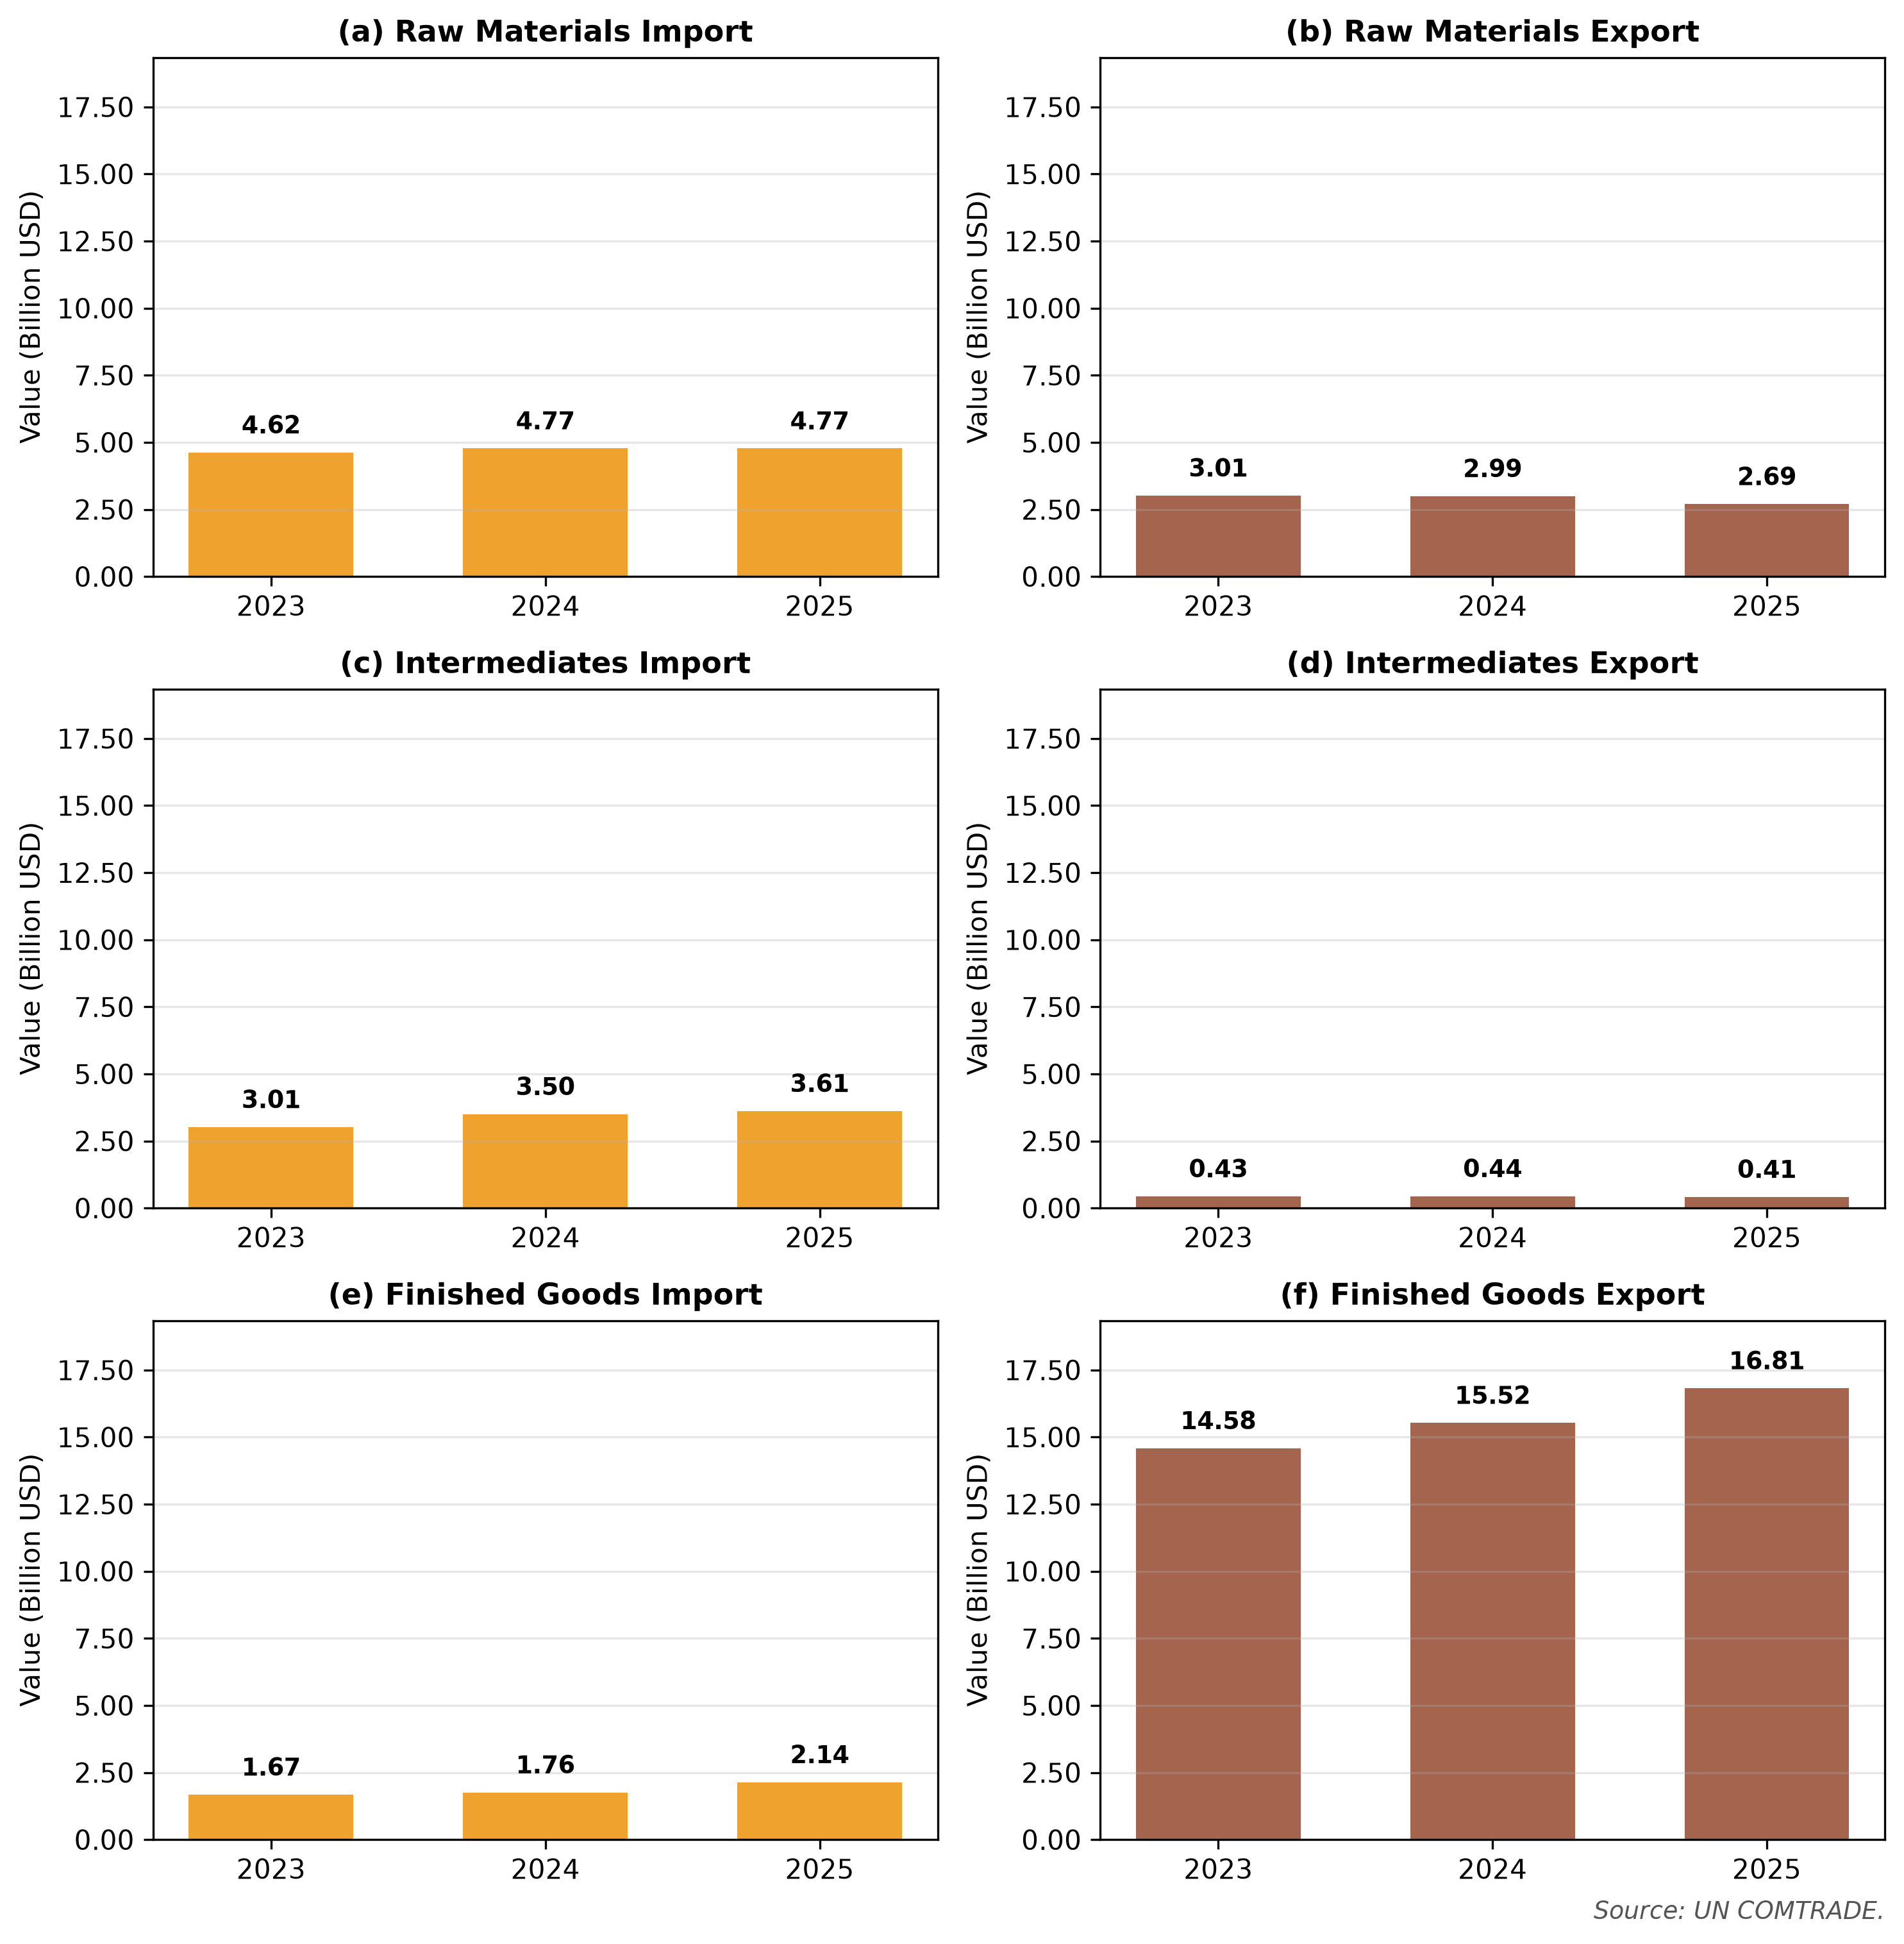
\includegraphics[width=0.75\linewidth,height=\textheight,keepaspectratio]{fig/trade_by_type.png}

}

\caption[\label{fig-trade}Exports and imports of textile and
footwear-related goods. Each panel shows
Indonesia's trade value in billion USD by year, split by product stage
(raw materials, intermediates, finished goods) and flow (import,
export). Source: UN COMTRADE.]{\label{fig-trade}Exports and imports of textile and
footwear-related goods\footnotemark{}. Each panel shows
Indonesia's trade value in billion USD by year, split by product stage
(raw materials, intermediates, finished goods) and flow (import,
export). Source: UN COMTRADE.}

\end{figure}%
\footnotetext{Raw materials are defined as HS Code
  chapters 50--55; intermediate goods cover chapters 56, 58, 59, and 60;
  and finished goods encompass chapters 61--64.}

One explanation for this pattern is that different segments of the
industry often participate in different value chains. Domestic raw
material producers may already be integrated into international
production networks and supply overseas buyers, while domestic yarn and
fabric manufacturers may source inputs from suppliers designated by
their clients or brand principals abroad. These relationships are often
highly specialized and not easily substitutable. As a result, trade
statistics alone cannot fully capture the degree of integration within
the industry, and policies based solely on HS-code classifications risk
disrupting established value chains.\footnote{This is also an issue in
  other industries that rely on global value chains, such as the food
  and beverage, machinery, and electronics industries (Gupta, Pane, and
  Pasaribu 2022; Hasran, Gupta, and Aaron 2025).}

The second implication of this economic dualism is that different
segments of the industry often require different policy responses. Firms
integrated into global value chains typically operate under a distinct
set of opportunities and constraints compared to domestically oriented
producers. Lead firms and global brands play an important coordinating
role by providing market access, setting production standards,
facilitating knowledge transfer, and reducing commercial risks faced by
suppliers (Gereffi, Humphrey, and Sturgeon 2005; Fernandez-Stark,
Frederick, and Gereffi 2011). Many export-oriented manufacturers also
benefit from stronger access to international markets, financing, and
production networks.

In contrast, domestically oriented textile and footwear firms operating
under their own brands tend to face greater challenges related to
financing, technology upgrading, productivity improvement, and market
expansion. Limited access to capital can constrain investment in new
machinery and production processes, while smaller scale often makes it
more difficult to meet the requirements needed to participate in global
value chains. Competition from imports, particularly illegal imports,
also remains a significant concern for these firms.

Differences are also evident across the production chain itself.
Upstream activities such as fiber production are highly capital and
energy-intensive, requiring substantial investment and sufficient
downstream demand to remain commercially viable. As a result, the number
of firms operating in these segments tends to be relatively limited.
Downstream manufacturing, particularly cut-make-trim (CMT) operations,
is generally more fragmented and less capital-intensive, allowing firms
to expand capacity incrementally as demand grows. Consequently, while
upstream competitiveness is often shaped by access to capital, energy,
and raw materials, downstream competitiveness depends more heavily on
labor availability, workforce skills, and productivity.

These differences highlight the importance of avoiding a
one-size-fits-all approach when addressing strategic issues in the
textile and footwear industry.

\subsection{International Trade}\label{international-trade}

Given the dual economic character and a highly global value chain-linked
industrial structure, international trade carries significant
implications for this industry. As discussed earlier, the US and the EU
remain the industry's most important export markets. Consequently,
developments in trade policy and market access in these economies have
significant implications for the industry's investment and production in
Indonesia.

For the US market, the primary challenges center on policy uncertainty
regarding tariffs and cost competitiveness. Indonesian industry is
vulnerable to reciprocal tariff threats and the potential loss of
Generalized System of Preferences (GSP) benefits, which would directly
raise import duties and compress margins. At the same time, Indonesia
faces intense competition from countries such as Vietnam, which is
highly competitive in terms of domestic production costs. The combined
pressure of tariff burdens and cost inefficiencies carries significant
potential to challenge exports and investment, underscoring the need for
structural transformation to enhance global competitiveness.

For the EU market, the outlook is more favorable. The conclusion in
substance of the Indonesia--European Union Comprehensive Economic
Partnership Agreement (IEU-CEPA) is expected to provide duty-free access
for Indonesian textile and footwear exports. This is particularly
important because it would place Indonesian exporters on a more level
playing field with competitors such as Vietnam, which already benefits
from preferential tariff access to the EU market.

However, access to these preferences depends on compliance with Rules of
Origin (RoO), particularly the ``double transformation'' requirement.
Under this rule, products must undergo at least two stages of production
within Indonesia to qualify for preferential tariffs. For garments, for
example, the fabric itself must also be produced domestically rather
than imported. The objective is to prevent transshipment and ensure that
tariff preferences are linked to genuine domestic value addition.

For firms operating under CMT (cut-make-trim) arrangements, this
requirement presents a significant challenge. Many manufacturers
continue to rely on imported fabrics and intermediate inputs supplied
through global buyer networks. Compliance with the double transformation
rule will therefore require either stronger domestic production of
intermediate goods or additional upstream investment by existing
suppliers.

While the double transformation requirement creates incentives to
strengthen domestic upstream and intermediate industries, imports are
likely to remain an important part of the industry's production
structure. This is particularly true for specialized inputs, proprietary
materials, and products that are not available domestically in the
required quality, specification, or volume. As a result, imports play a
dual role within the industry. On one hand, they can compete directly
with domestic producers in the same segment. On the other, they provide
access to inputs that support production, exports, and participation in
global value chains. Studies by DEN, Gherzi and Prospera similarly
emphasize that imports can both support and challenge industrial
development.

The more immediate concern is not legal imports themselves, but illegal
imports that circumvent import duties and regulatory requirements
altogether. In August 2025, a joint operation by the Ministry of Trade,
the State Intelligence Agency (BIN), and the Strategic Intelligence
Agency of the Indonesian National Armed Forces (BAIS TNI) seized 19,391
bales of illegal textile imports valued at IDR 112.35 billion (Deviyana
2025). Industry studies suggest that such practices commonly involve
underreporting, underinvoicing, and the use of unofficial entry points.
Beyond reducing government revenue, illegal imports undermine fair
competition and weaken the competitiveness of domestic firms.

\subsection{Sustainability Issues}\label{sustainability-issues}

In addition to trade-related issues, sustainability is becoming an
increasingly important issue for the textile and footwear industry. This
is especially relevant for companies that export to the EU markets,
where sustainability requirements are gradually becoming part of market
access requirements.

Under the European Green Deal, the European Union has introduced a
number of regulations to encourage more sustainable production and
consumption patterns. One of the most important for the textile and
footwear industry is the Ecodesign for Sustainable Products Regulation
(ESPR), which entered into force in 2024 and is currently undergoing
further consultation and implementation (Yan 2025; European Commission
2024).

The ESPR includes requirements related to product durability,
repairability, recyclability, and traceability. One key element is the
Digital Product Passport (DPP), which requires information on a
product's origin, material composition, production process, and
environmental footprint to be traceable throughout the value chain
(Costa 2025). Meeting these requirements will require firms to
strengthen data collection, traceability systems, and digitalization
across their operations.

The implications extend beyond firms directly exporting to the European
Union. Because traceability requirements apply throughout the value
chain, upstream suppliers are also likely to be affected. This is
particularly relevant in the textile industry, where fiber and fabric
production is highly capital-intensive and characterized by significant
economies of scale. Rather than operating separate production systems
for different markets, many producers may find it more practical to
adopt these standards across their entire operations.

Several export-oriented manufacturers have already begun adapting to
these changes. One fiber and fabric factory in Central Java\footnote{To
  preserve the confidentiality of commercially sensitive information,
  the company name is not disclosed. The information is based on an
  in-depth interview conducted by DEN with an export-oriented fiber and
  fabric manufacturer in Central Java in 2025.} has already developed a
real-time dashboard system ready to be integrated with systems such as
the DPP. The company has also transitioned its entire energy production
to biomass.

The transition to greener production, however, remains challenging in
Indonesia. While industrial energy costs are relatively competitive, the
country's energy system continues to rely heavily on fossil fuels.
Manufacturers seeking to reduce their carbon footprint may invest in
alternative energy sources such as biomass, solar power, or natural gas,
yet each faces its own constraints, including limited biomass
availability, regulatory restrictions on solar deployment, and gaps in
gas supply and infrastructure.

For many firms, sustainability is no longer solely an environmental
issue. Increasingly, it is becoming a business requirement linked to
export competitiveness and participation in global value chains.

\subsection{Technology}\label{technology}

Technology adoption remains an important determinant of competitiveness
in Indonesia's textile \& garments and footwear industry. Beyond
reducing production costs, technological upgrading is increasingly
necessary to improve productivity, product quality, and operational
efficiency in an increasingly competitive global market.

Figure~\ref{fig-machinery} illustrates that Indonesia has generally
lagged behind regional competitors such as Vietnam in machinery
modernization, particularly in spinning and weaving. Over the past
decade, Indonesia experienced declining capacity in several upstream
segments, including ring spinning, open-end spinning, and shuttleless
looms, while Vietnam continued to expand capacity through sustained
investment in newer production equipment. This trend suggests that the
challenge facing Indonesia is not only one of competitiveness, but also
of maintaining productive capacity in strategic upstream segments of the
textile value chain.

\begin{figure}[htbp!]

\centering{

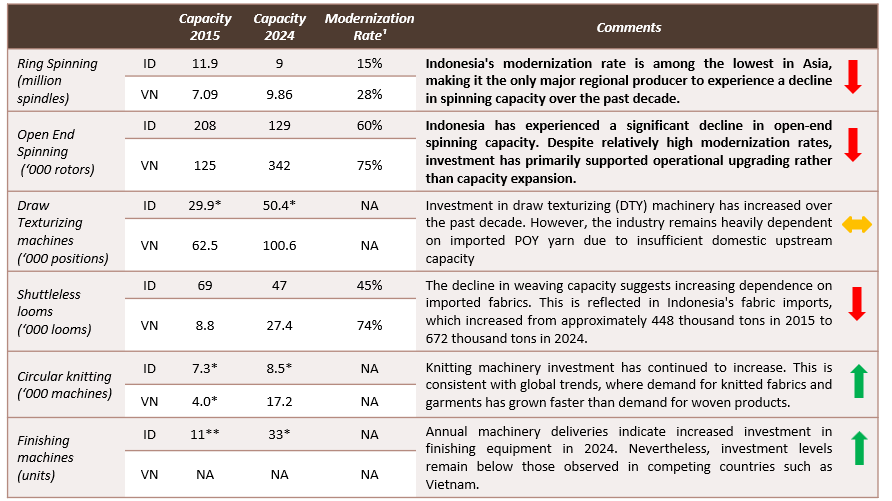
\includegraphics[width=0.9\linewidth,height=\textheight,keepaspectratio]{fig/machinery_modernization.png}

}

\caption{\label{fig-machinery}Comparison of textile machinery
modernization in Indonesia and Vietnam. Source: DEN, ITMF, Gherzi.}

\end{figure}%

Older machinery tends to be less productive, more energy-intensive, and
more costly to maintain, reducing competitiveness relative to producers
that have invested in newer technologies. As a result, machinery
modernization remains one of the industry's most pressing priorities,
particularly for upstream segments that form the foundation of domestic
textile value chains.

Automation is also becoming increasingly important, not necessarily as a
substitute for labor, but as a means of improving productivity, quality
consistency, and operational efficiency. Several large manufacturers
have adopted automated cutting equipment, material handling systems, and
warehouse management technologies to reduce production bottlenecks and
improve process control. Interviews conducted by DEN with
export-oriented manufacturers suggest that automation has helped reduce
defect rates, improve product consistency, and enhance production
efficiency, all of which are critical for meeting the quality
requirements of global buyers\footnote{Based on interviews conducted by
  DEN with export-oriented textile manufacturers in 2025. Company names
  are not disclosed to preserve the confidentiality of commercially
  sensitive information.}. While broader adoption remains uneven,
particularly among smaller firms, automation is likely to become an
increasingly important component of industrial upgrading in the years
ahead.

\subsection{Workforce Readiness}\label{workforce-readiness}

The textile, garment, and footwear industries remain among Indonesia's
most important manufacturing employers. Total employment increased from
4.1 million workers in 2020 to more than 5.0 million in 2025, equivalent
to approximately one-quarter of formal manufacturing employment
nationwide (BPS 2025a). Textile and garment manufacturing continues to
dominate employment within the sector, accounting for nearly four
million workers in 2025. Nevertheless, the fastest employment growth
occurred in the footwear industry, where the workforce expanded by
around 60 percent between 2020 and 2025, compared with approximately
15--20 percent growth in textile and garment manufacturing in the same
period (Figure~\ref{fig-workers}).

\begin{figure}[H]

\centering{

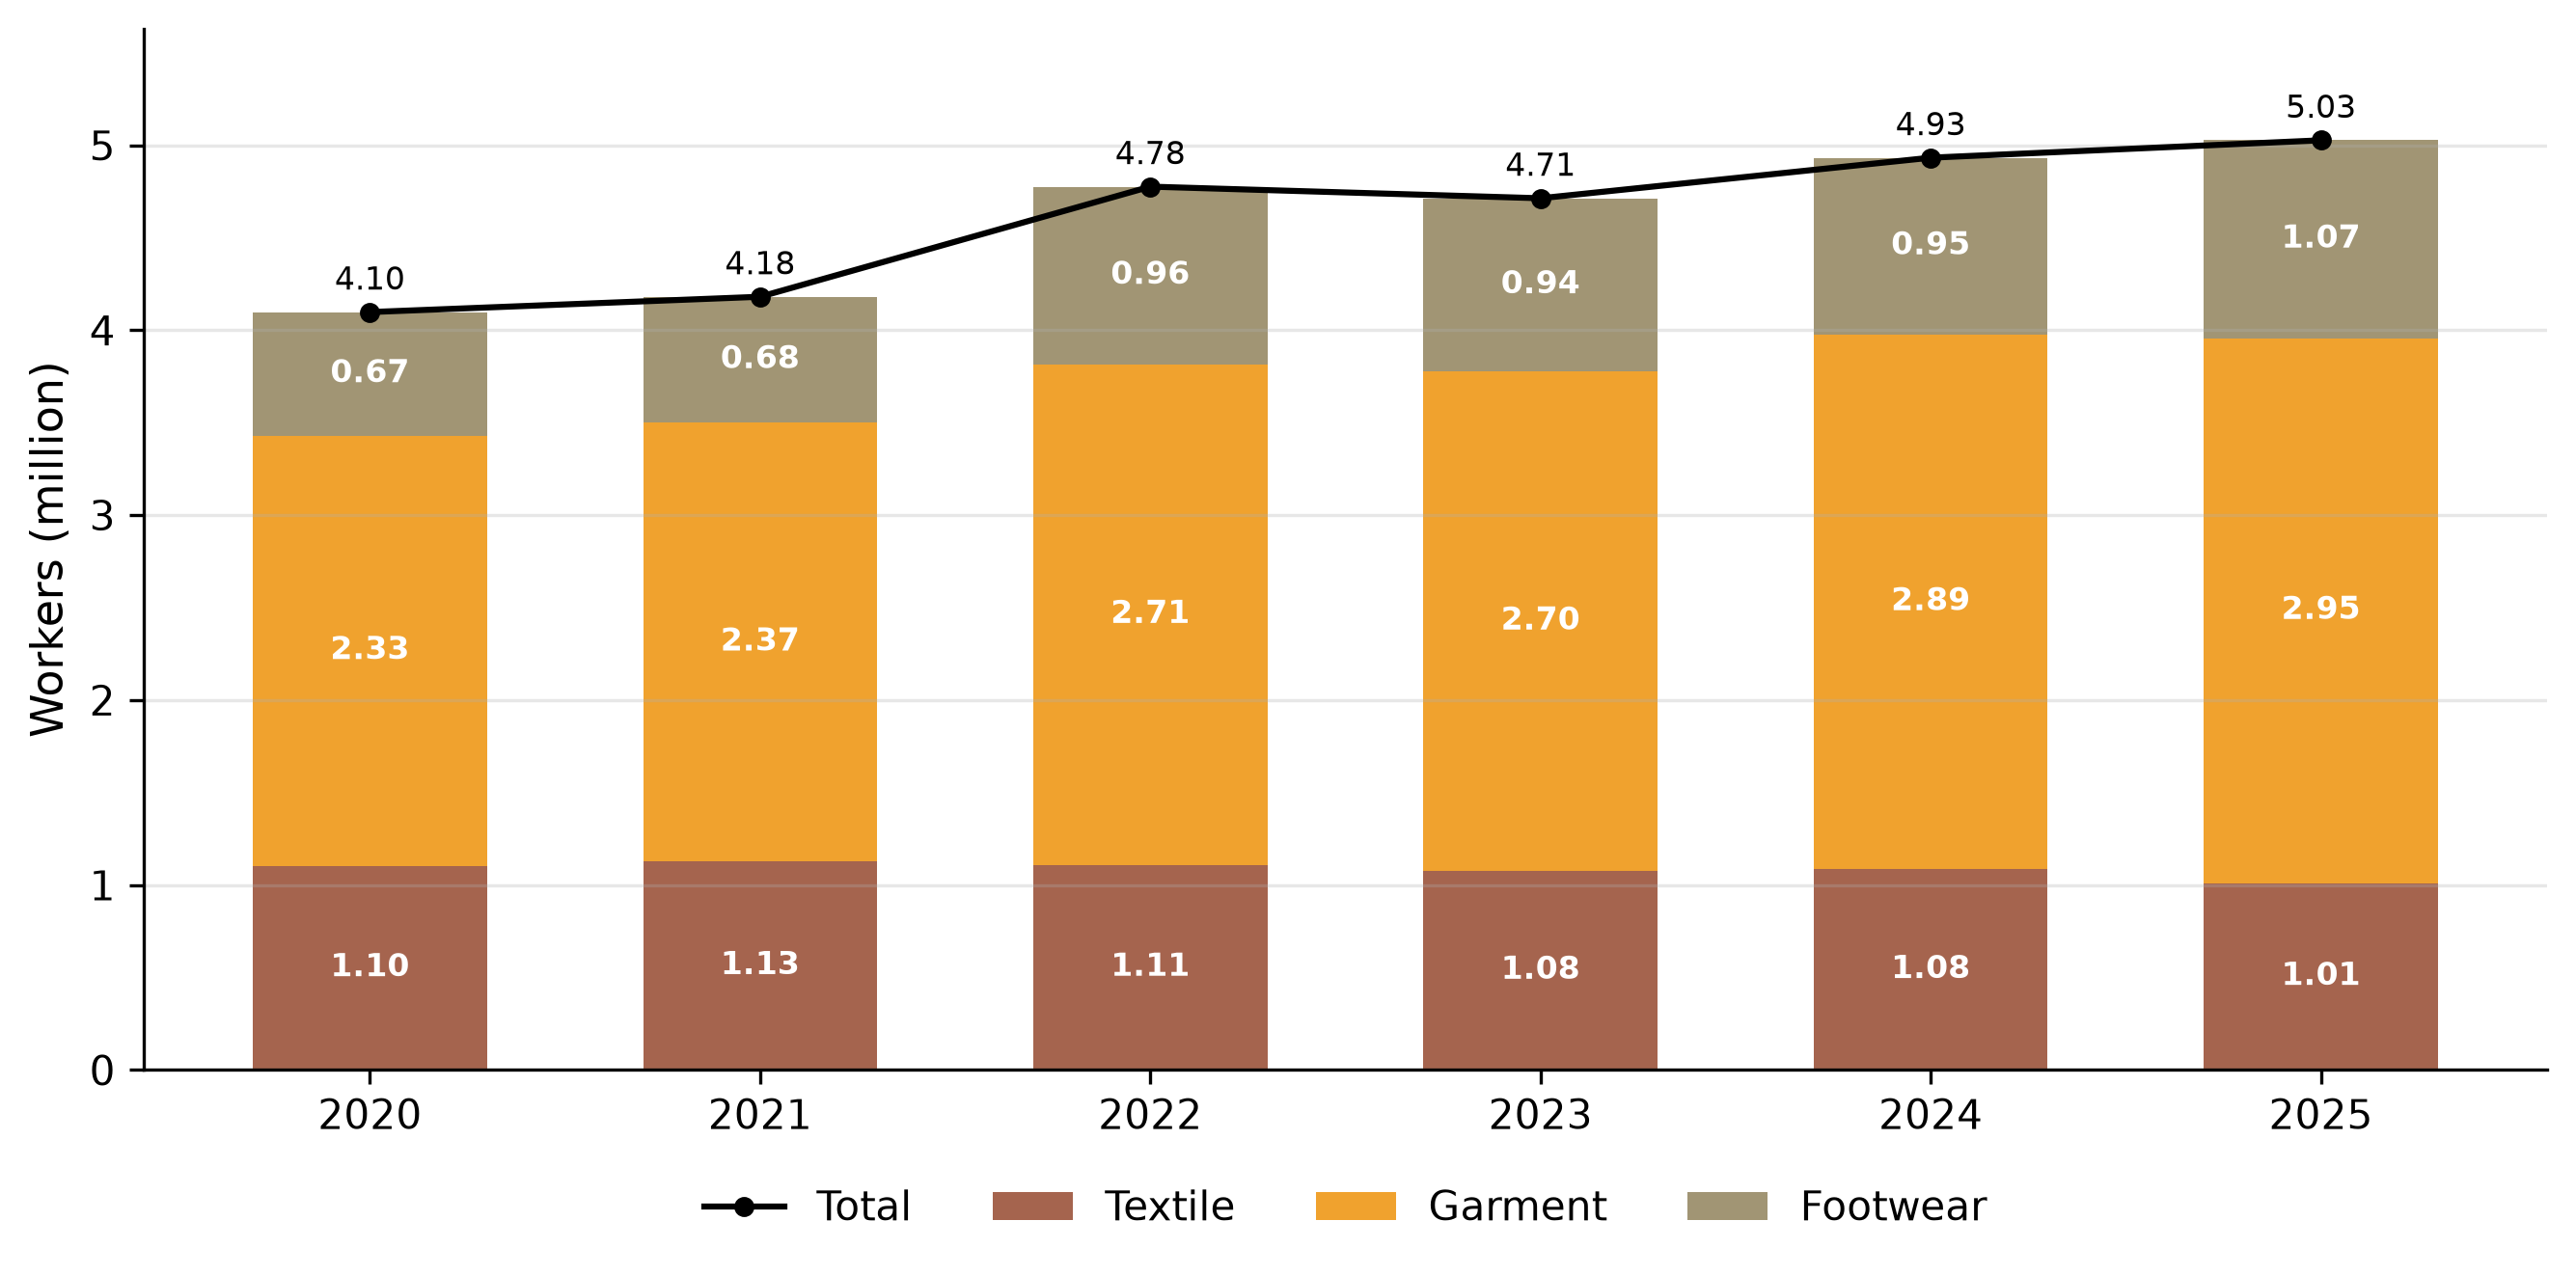
\includegraphics[width=0.7\linewidth,height=\textheight,keepaspectratio]{fig/workers.png}

}

\caption{\label{fig-workers}Number of workers in Indonesia's
labor-intensive industries (million), 2020--2025. Source: BPS,
Sakernas.}

\end{figure}%

The growth in employment naturally raises concerns about whether labor
supply can keep pace with industry demand. However, available workforce
projections suggest that Indonesia is unlikely to face a shortage of
workers for either industry. According to projections from the Ministry
of Manpower, the annual supply of vocational graduates (SMK and
Vocational graduates) relevant to the textile and footwear industries is
expected to continue growing through 2029. For textiles and garments,
the supply of graduates is projected to increase from approximately
624,802 in 2025 to 765,763 in 2029, equivalent to average annual growth
of 5.2 percent. Footwear-related graduates are projected to rise from
around 133,232 to approximately 183 thousand over the same period,
representing annual growth of 8.3 percent (Figure~\ref{fig-workforce}).

\begin{figure}[htbp!]

\centering{

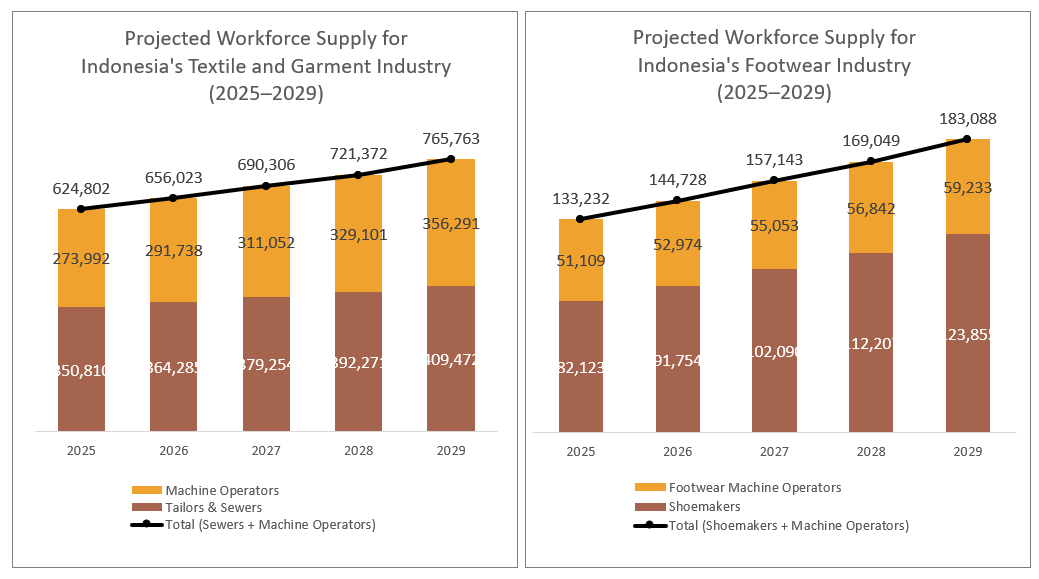
\includegraphics[width=0.95\linewidth,height=\textheight,keepaspectratio]{fig/workforce_projection.png}

}

\caption[\label{fig-workforce}Projected workforce supply for Indonesia's
textile \& garment, and footwear industries. Source: Ministry of Manpower.]{\label{fig-workforce}Projected workforce supply for Indonesia's
textile \& garment, and footwear industries\footnotemark{}. Source: Ministry of Manpower.}

\end{figure}%
\footnotetext{Labor Supply
  Projections for Vocational Education and Training Graduates (SMK and
  Diploma).}

These projected graduate numbers substantially exceed estimated labor
demand associated with recent investment activity. Data collected for
this study indicate that 27 newly established textile and footwear
factories are expected to generate employment in 2025--2026 for
approximately 108,000 workers. Against an annual vocational graduate
pipeline exceeding 750,000 individuals in 2025, this suggests that labor
availability is unlikely to be a binding constraint for either industry
in the near term.

Rather, the more important issue appears to be workforce productivity
and job readiness. Discussions with industry stakeholders indicate that
substantial productivity differences exist across production locations.
Footwear manufacturers operating in established industrial clusters in
Tangerang, for example, reported significantly higher output per worker
than newer facilities in Central Java. Productivity data shared during
consultations suggest a range of approximately 1.6 to nearly 5.0 pairs
of shoes produced per worker per day. Industry participants attributed
much of this variation to differences in workforce experience, factory
learning curves, supervisory capabilities, and operational maturity.

As newer facilities gain experience and refine their production
processes, part of the productivity gap observed should be narrowed over
time. Nevertheless, these findings underscore the importance of
workforce readiness and skills development in enabling new production
centers to translate labor availability into productivity gains as
investment continues to expand.

As previously discussed, Indonesia's position within the textile and
garment, and footwear value chains is concentrated in manufacturing and
assembly activities. Therefore, competitiveness depends heavily on
production efficiency and consistency rather than on capital-intensive
upstream capabilities or brand-driven downstream value. Meanwhile,
within this segment of the value chain, workforce productivity can be
influenced directly through domestic policy, for example through SMK
curriculum reforms.

Given that SMK represent the primary pipeline of vocational graduates
entering the textile and garment, and footwear industries, the
productivity gap observed raises an important policy question: whether
current vocational curricula are sufficiently aligned with industry
requirements and the production environment that the graduates are
expected to enter. This warrants closer examination, including the
extent to which textile and garment-related vocational tracks are
oriented towards industrial, line-based production processes as opposed
to individual or small-batch production models. Notably, as of 2026,
footwear does not constitute a standalone vocational program
(\emph{jurusan}) within the SMK system. It is instead taught as a module
within the broader Leather and Synthetic Leather Craftsmanship
curriculum, despite footwear's distinct production processes and its
status as a significant export-oriented industry.

Addressing this alignment, such as through closer collaboration between
vocational institutions and industry in curriculum development, will
likely be necessary to ensure that the strong quantitative growth in
labor supply translates into a workforce capable of meeting the
productivity standards required to sustain Indonesia's competitiveness
in global textile and garment, and footwear value chains.

\section{Government Policies and Support
Programs}\label{government-policies-and-support-programs}

The Indonesian government has introduced a range of policies affecting
the textile and footwear industry, covering trade, investment, machinery
modernization, and workforce development.

On the trade front, Permendag No.~17/2025 introduced import requirements
for a range of textile products, including Import Approvals (Persetujuan
Impor) and Surveyor Reports (Laporan Surveyor). The regulation aims to
strengthen oversight of textile imports while balancing the needs of
domestic industry and downstream users. This was followed by Permenperin
No.~27/2025, which governs the issuance of technical considerations
(pertimbangan teknis/pertek) for textile imports, particularly to ensure
the availability of raw materials for domestic manufacturing activities.

Indonesia also continues to utilize trade remedy instruments in the
textile sector, including anti-dumping duties (BMAD) and safeguard
measures (BMTP) on selected products. Long-standing measures include
anti-dumping duties on imports of Polyester Staple Fiber from India,
China, and Taiwan, as well as spin drawn yarn from China. More recently,
additional anti-dumping and safeguard measures have been applied to
products such as woven cotton fabrics and cotton yarn through PMK
48/2024, PMK 67/2025, and PMK 98/2025. These measures are intended to
address unfair trade practices and import surges that may adversely
affect domestic producers. Their impact, however, varies across segments
of the industry. While they may provide additional protection for
domestic manufacturers competing directly with imports, they can also
increase input costs for firms that rely on imported raw materials and
intermediate goods.

The government has also introduced a range of incentives to promote
investment across the textile and footwear value chain. These include
import duty facilities for machinery and equipment under PMK 179/2009,
tax incentives for new investments in labor-intensive industries under
PMK 16/2020, and tax holiday facilities under PMK 130/2020 for eligible
pioneer industries. Several of these incentives are also relevant to
upstream industries, including basic chemical manufacturing, which plays
an important role in the production of synthetic fibers and other
textile inputs.

On workforce development, the government has introduced incentives to
support apprenticeship programs, workforce training, and research
activities through the super deduction tax scheme under PMK 128/2019 and
PMK 153/2020. Additional support has also been provided to
labor-intensive industries, including the textile and footwear sector,
through government-borne income tax facilities under PMK 10/2025 and PMK
105/2025.

To support machinery modernization, the government currently operates
two complementary programs. The first is the Machinery and Equipment
Restructuring Program (Permenperin 20/2024), which provides partial
reimbursement for the purchase of new production machinery and
equipment. Under the 2026 program, firms may receive reimbursement of up
to 25 percent of the purchase value for domestically produced machinery
and 10 percent for imported machinery, subject to a maximum
reimbursement of IDR 500 million per company. The second is the
Labor-Intensive Reinvestment Incentive Program (KIPK), which provides a
5 percent interest subsidy on investment loans ranging from IDR 500
million to IDR 10 billion. Industry stakeholders generally view these
programs as positive steps toward supporting industrial modernization
but have identified several implementation challenges, including
relatively limited reimbursement ceilings, the exclusion of supporting
equipment, and eligibility requirements that may constrain
participation.

\subsection{Regulatory Reform as a Driver of Industrial
Competitiveness}\label{regulatory-reform-as-a-driver-of-industrial-competitiveness}

Achieving that export ambition will depend not only on financing and
incentives, but equally on the speed at which investment commitments can
be translated into operational factories and employed workers. Two
regulatory areas are particularly relevant in this regard: business
licensing (perizinan berusaha) and technical import approvals (pertek
impor) for industrial raw materials. Steps have been taken on both
fronts, though the degree to which they deliver on their intent will
hinge on consistent and measurable implementation across agencies and
regions.

Firstly, on the business licensing front, DEN's engagement with textile
and garment sector players across West Java, Central Java, Banten, and
East Java identified 27 companies totalling 108,179 workers whose
investment realization timelines are sensitive to permitting duration
(Figure~\ref{fig-pipeline}).

\begin{figure}[htbp!]

\centering{

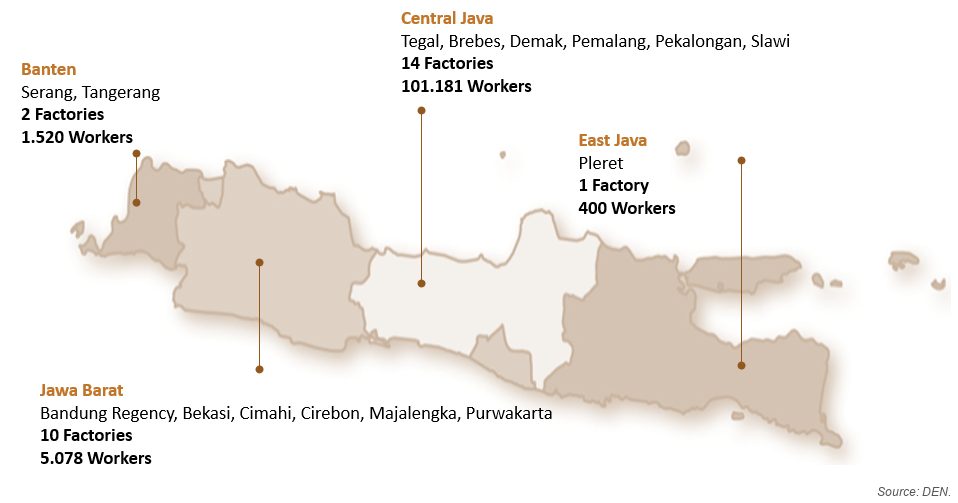
\includegraphics[width=1\linewidth,height=\textheight,keepaspectratio]{fig/investment_pipeline.png}

}

\caption{\label{fig-pipeline}Pipeline of textile, garment \& footwear
investments (2025--2026). Source: DEN.}

\end{figure}%

A deeper look at one footwear facility in Central Java employing 12,000
workers illustrates the extent to which permitting delays can constrain
investment realization. The AMDAL (environmental permit) process alone
took approximately 1,095 days, accounting for the majority of the
project's licensing timeline (Figure~\ref{fig-licensing}).

\begin{figure}[htbp!]

\centering{

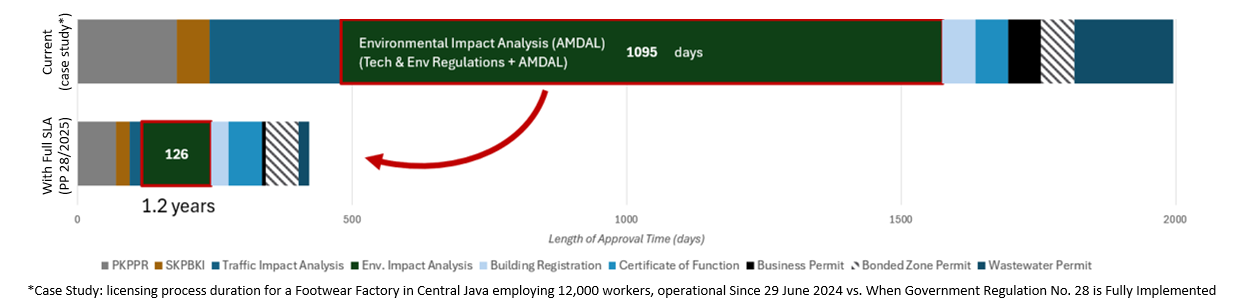
\includegraphics[width=1\linewidth,height=\textheight,keepaspectratio]{fig/licensing_time.png}

}

\caption{\label{fig-licensing}Potential reduction in investment approval
time through full implementation of PP No.~28/2025. Source: DEN.}

\end{figure}%

While this case is illustrative rather than representative, similar
challenges have been reported across the sector. Government Regulation
No.~28 of 2025 seeks to address these bottlenecks by introducing Service
Level Agreements (SLAs) with defined processing timelines for each
approval stage. Full implementation could reduce total licensing time
from 2--3 years to approximately 1.2 years, including a reduction in
AMDAL processing time from 1,095 days to 126 days. The effectiveness of
these reforms will ultimately depend on consistent enforcement and
strong coordination across all levels of government.

Secondly, beyond business licensing, the efficiency of import approval
processes remains an important factor affecting investment realization
and industrial competitiveness. In this context, Satgas P3-MPPE,
established under Presidential Decree No.~4 of 2026 and coordinated by
the Coordinating Ministry for Economic Affairs, has identified the
simplification of technical import approvals for industrial raw
materials as an early reform priority. The initiative includes
adjustments to technical approval requirements under the Ministry of
Industry as well as related trade policy revisions under the Ministry of
Trade.

For the textile and footwear sectors, these reforms are particularly
relevant. Manufacturers rely on timely access to specialized fibers,
yarns, chemicals, and other intermediate inputs that are often specified
by global buyers and brand principals. Delays in obtaining technical
import approvals or clearing imported materials can disrupt production
schedules, increase operating costs, and reduce supply chain
reliability.

The issue is becoming increasingly important as Indonesia expands its
upstream textile capacity through new yarn and fabric investments. These
facilities will play a critical role in enabling compliance with the
IEU-CEPA double transformation requirement, making efficient import
administration an important complement to broader industrial development
efforts.

Taken together, reforms in business licensing and import approvals
address two regulatory areas that directly influence the pace of
investment realization in the textile and footwear sector. If
implemented effectively, these measures could accelerate project
execution, strengthen investor confidence, and support faster job
creation. Indonesia has already introduced many of the necessary policy
instruments; the key challenge now lies in ensuring consistent
implementation across institutions and levels of government.

\section{Conclusion}\label{conclusion}

Indonesia's textile and footwear industries remain strategically
important not only because of their contribution to exports, but also
because of their role as one of the country's largest sources of formal
manufacturing employment. The industries are well positioned to benefit
from several favorable developments, including the diversification of
global sourcing away from China, growing investor interest in Southeast
Asia, and the conclusion in substance of the Indonesia--European Union
Comprehensive Economic Partnership Agreement (IEU-CEPA). Together, these
developments create a window of opportunity for Indonesia to strengthen
its position within global textile and footwear value chains.

The findings of this study suggest that Indonesia's competitiveness
challenge is not primarily a matter of production costs. Relative to
major competitor countries, Indonesia remains broadly competitive in
labor, energy, and water costs. Instead, the more significant
constraints relate to investment realization, technology upgrading,
workforce productivity, and the ability to meet increasingly demanding
market requirements, particularly those related to sustainability and
traceability.

The study also highlights the importance of recognizing the industry's
structural diversity. Indonesia's textile and footwear sectors consist
of both globally integrated manufacturers linked to international buyers
and domestically oriented producers serving local markets. Differences
also exist across the value chain itself, with upstream segments facing
challenges related to capital intensity, scale, and raw material
availability, while downstream segments depend more heavily on labor
productivity, operational efficiency, and market access. As a result,
policy interventions need to be tailored to the specific constraints
faced by different segments rather than relying on a uniform approach.

In the near term, improving the speed and predictability of investment
realization should be a policy priority. Evidence collected in this
study indicates that lengthy licensing processes and administrative
bottlenecks can significantly delay factory construction and employment
creation. Ongoing reforms to business licensing and import approval
procedures therefore have the potential to generate substantial economic
benefits by accelerating investment implementation, strengthening
investor confidence, and supporting job creation.

Over the longer term, Indonesia's ability to capture greater value from
the textile and footwear industries will depend on strengthening the
domestic industrial ecosystem and improving productivity. While
workforce projections suggest that labor supply is unlikely to be a
binding constraint, significant productivity gaps remain across
production locations, highlighting the importance of workforce
readiness, vocational education, and industry-relevant skills
development. At the same time, continued investment in machinery
modernization, sustainability compliance, and upstream industrial
capabilities will be necessary to increase domestic value added and
support compliance with evolving global market requirements.

Ultimately, Indonesia's opportunity is not simply to attract more
textile and footwear investment, but to deepen its participation in
global value chains while increasing the domestic value created from
that participation. Achieving this objective will require a coordinated
approach that combines regulatory reform, industrial upgrading,
workforce development, and ecosystem building. If these challenges can
be addressed effectively, the textile and footwear industries can remain
an important source of export growth, formal employment, and industrial
transformation in the years ahead.

\section*{Reproducibility Statement}\label{reproducibility-statement}
\addcontentsline{toc}{section}{Reproducibility Statement}

The source files for this paper are hosted at
\url{https://github.com/imedkrisna/tekstil}. All data-driven figures
(Figure~\ref{fig-growth}, Figure~\ref{fig-recovery},
Figure~\ref{fig-investment}, Figure~\ref{fig-globalimport},
Figure~\ref{fig-smile}, Figure~\ref{fig-trade},
Figure~\ref{fig-workers}) are generated by the Jupyter notebook
\texttt{fig/fig.ipynb} from the Excel files in the \texttt{fig/} folder;
the Sakernas employment counts behind Figure~\ref{fig-workers} are
entered directly in the notebook. The market shares in
Table~\ref{tbl-shares} are computed in the same notebook from bilateral
UN COMTRADE data (\texttt{TradeData.xlsx}), which is not redistributed
in the repository; the notebook preserves the computed output. The
remaining figures (value chain diagrams, maps, and charts based on DEN
fieldwork and third-party databases) are included as static images in
\texttt{fig/}; the two maps were cropped from the originals, which are
kept in the same folder with an \texttt{\_original} suffix.

\phantomsection\label{refs}
\begin{CSLReferences}{1}{1}
\bibitem[\citeproctext]{ref-aprayon2024}
Asia Pacific Rayon. 2024. \emph{Sustainability Report 2024: Clean
Manufacturing at the Forefront}. Asia Pacific Rayon.
\url{https://www.aprayon.com/id/keberlanjutan/dasbor-keberlanjutan/}.

\bibitem[\citeproctext]{ref-adb2025mrio}
Asian Development Bank. 2025. \emph{ADB Multiregional Input-Output
Tables at Current Prices}.
\url{https://kidb.adb.org/globalization/current}.

\bibitem[\citeproctext]{ref-bps2025sakernas}
BPS. 2025a. \emph{Booklet Sakernas Februari 2025}. Vol. 8. BPS.
\url{https://www.bps.go.id/id/publication/2025/07/14/90a6b20c25c63176d23ab46c/booklet-sakernas-februari-2025.html}.

\bibitem[\citeproctext]{ref-bps2025tpt}
BPS. 2025b. \emph{Tingkat Pengangguran Terbuka Menurut Provinsi
(Persen), 2024--2025}.
\url{https://www.bps.go.id/id/statistics-table/2/NTQzIzI=/tingkat-pengangguran-terbuka-menurut-provinsi.html}.

\bibitem[\citeproctext]{ref-costa2025dpp}
Costa, Antonio Braz. 2025. \emph{Digital Product Passport Impacts on the
Global Supply Chain and Technology Requirements}. ITMF Annual Conference
\& IAF World Fashion Convention, Yogyakarta.
\url{https://www.itmf-iaf-conference-2025-yogyakarta.org/conference-downloads-25}.

\bibitem[\citeproctext]{ref-deviyana2025}
Deviyana, Nia. 2025. {``19 Ribu Bal Pakaian Bekas Diduga Impor Ilegal
Diamankan, Nilainya Rp112 Miliar.''} \emph{IDXChannel}, 2025.
\url{https://www.idxchannel.com/news/19-ribu-bal-pakaian-bekas-diduga-impor-ilegal-diamankan-nilainya-rp112-miliar}.

\bibitem[\citeproctext]{ref-ec2024espr}
European Commission. 2024. \emph{Ecodesign for Sustainable Products
Regulation}.
\url{https://commission.europa.eu/energy-climate-change-environment/standards-tools-and-labels/products-labelling-rules-and-requirements/ecodesign-sustainable-products-regulation_en}.

\bibitem[\citeproctext]{ref-feenstra2021}
Feenstra, Robert C., and Alan M. Taylor. 2021. \emph{International
Macroeconomics}. 5th ed. Worth.

\bibitem[\citeproctext]{ref-fernandezstark2011}
Fernandez-Stark, Karina, Stacey Frederick, and Gary Gereffi. 2011.
\emph{The Apparel Global Value Chain: Economic Upgrading and Workforce
Development}. Center on Globalization, Governance \& Competitiveness.

\bibitem[\citeproctext]{ref-gereffi2010}
Gereffi, Gary, and Stacey Frederick. 2010. \emph{The Global Apparel
Value Chain, Trade and the Crisis: Challenges and Opportunities for
Developing Countries}. World Bank.
\url{https://doi.org/10.1596/1813-9450-5281}.

\bibitem[\citeproctext]{ref-gereffi2005governance}
Gereffi, Gary, John Humphrey, and Timothy Sturgeon. 2005. {``The
Governance of Global Value Chains.''} \emph{Review of International
Political Economy} 12 (1): 78--104.

\bibitem[\citeproctext]{ref-goto2023}
Goto, Kenta. 2023. {``Viet Nam's Textile and Garment Industry in the
Global Value Chain.''} In \emph{Viet Nam 2045: Development Issues and
Challenges}. ERIA.
\url{https://www.eria.org/uploads/16_ch_12-Textile-and-Garment-Industry-in-GVC.pdf}.

\bibitem[\citeproctext]{ref-gupta2022gvc}
Gupta, Krisna, Irma Tsuraya Choirinnida, and Muhammad Taufik. 2022.
{``Global Value Chain Impact for Indonesia Economy and the Way to Make
It More Resilient.''} In \emph{Indonesia Post-Pandemic Outlook:
Rethinking Health and Economics Post-COVID-19}. Sustainable Indonesia.
Penerbit BRIN. \url{https://penerbit.brin.go.id/press/catalog/book/537}.

\bibitem[\citeproctext]{ref-gupta2022neraca}
Gupta, Krisna, Deasy Pane, and Donny Pasaribu. 2022. {``The Advent of a
New Trade Governance After the Omnibus Law: Neraca Komoditas.''}
\emph{CIPS Policy Paper} 47.
\url{https://www.cips-indonesia.org/publications/the-advent-of-a-new-trade-governance-after-the-omnibus-law\%3A-neraca-komoditas?lang=id}.

\bibitem[\citeproctext]{ref-hasran2025}
Hasran, Krisna Gupta, and Rasya Athalla Aaron. 2025. {``Dampak Sistem
Neraca Komoditas Terhadap Birokrasi Perdagangan Dan Harga Pangan Di
Indonesia.''} \emph{CIPS Policy Paper} 44.
\url{https://www.cips-indonesia.org/publications/dampak-sistem-neraca-komoditas-terhadap-birokrasi-perdagangan-dan-harga-pangan-di-indonesia?lang=id}.

\bibitem[\citeproctext]{ref-hodrick1997}
Hodrick, Robert J., and Edward C. Prescott. 1997. {``Postwar u.s.
Business Cycles: An Empirical Investigation.''} \emph{Journal of Money,
Credit and Banking} 29 (1): 1--16.
\url{https://doi.org/10.2307/2953682}.

\bibitem[\citeproctext]{ref-kartasasmita2025}
Kartasasmita, Agus Gumiwang. 2025. \emph{Keynote Speech by the Minister
of Industry}. ITMF Annual Conference \& IAF World Fashion Convention,
Yogyakarta.
\url{https://www.itmf-iaf-conference-2025-yogyakarta.org/conference-downloads-25}.

\bibitem[\citeproctext]{ref-kemenko2025}
Kemenko Perekonomian. 2025. \emph{Pemerintah Tingkatkan Penguatan Akses
Pembiayaan Produktif Dengan Kredit Alsintan Dan Kredit Industri Padat
Karya}. Siaran Pers HM.02.04/287/SET.M.EKON.3/08/2025.
\url{https://www.ekon.go.id/publikasi/detail/6527/pemerintah-tingkatkan-penguatan-akses-pembiayaan-produktif-dengan-kredit-alsintan-dan-kredit-industri-padat-karya}.

\bibitem[\citeproctext]{ref-kemenkeu2024}
Kementerian Keuangan. 2024. \emph{APBN Kita: Kinerja Dan Fakta, Oktober
2024}. Kementerian Keuangan.
\url{https://media.kemenkeu.go.id/getmedia/4924fc3f-9748-4530-8757-dd7a123b4c73/APBN-KiTa-Oktober-2024.pdf?ext=.pdf}.

\bibitem[\citeproctext]{ref-kemenkeu2025}
Kementerian Keuangan. 2025. \emph{Laporan Belanja Perpajakan 2024}.
Kementerian Keuangan.
\url{https://fiskal.kemenkeu.go.id/publikasi/tax-expenditure-report}.

\bibitem[\citeproctext]{ref-kumparan2026}
KumparanBISNIS. 2026. {``Fakta-Fakta Pembentukan BUMN Tekstil Dengan
Modal Rp 101 t.''} \emph{Kumparan}, 2026.
\url{https://kumparan.com/kumparanbisnis/fakta-fakta-pembentukan-bumn-tekstil-dengan-modal-rp-101-t-26dtdGAXO6Z/full}.

\bibitem[\citeproctext]{ref-lubis2025}
Lubis, Daniel Bastian. 2025. \emph{Keadaan Ketenagakerjaan Agustus
2025}. Workshop Penyusunan Laporan Tahunan Dewan Ekonomi Nasional,
Bogor.

\bibitem[\citeproctext]{ref-masitoh2024}
Masitoh, Siti. 2024. {``Tekstil Banyak Menikmati Fasilitas Kawasan
Berikat.''} \emph{Kontan}, 2024.
\url{https://insight.kontan.co.id/news/tekstil-banyak-menikmati-fasilitas-kawasan-berikat}.

\bibitem[\citeproctext]{ref-kemenperin2024}
Ministry of Industry. 2024. \emph{Peta Potensi Industri Alas Kaki Skala
Menengah \& Besar Di Indonesia 2024}. Balai Pemberdayaan Industri
Persepatuan Indonesia (BPIPI).
\url{https://datacenter-bpipi.kemenperin.go.id/}.

\bibitem[\citeproctext]{ref-kemenperin2025}
Ministry of Industry. 2025. \emph{Arah Program Dan Kegiatan Pengembangan
Sektor Industri Tekstil Dan Pakaian Jadi Tahun 2026--2029}. Forum
Kebijakan Strategis: {``Bedah Hasil Kajian Arah Pengembangan Industri
Tekstil dan Pakaian Jadi yang Berkelanjutan dan Berdaya Saing Global,''}
Jakarta.

\bibitem[\citeproctext]{ref-ramadhan2025}
Ramadhan, Gaffari. 2025. \emph{Navigating Uncertainty \& Adopting
Technology -- Pathways to Sustainable Strength in the Textile and
Apparel Industry}. ITMF Annual Conference \& IAF World Fashion
Convention, Yogyakarta.
\url{https://www.itmf-iaf-conference-2025-yogyakarta.org/conference-downloads-25}.

\bibitem[\citeproctext]{ref-razzak1997}
Razzak, W. 1997. {``The Hodrick-Prescott Technique: A Smoother Versus a
Filter: An Application to New Zealand GDP.''} \emph{Economics Letters}
57 (2): 163--168. \url{https://doi.org/10.1016/S0165-1765(97)00178-X}.

\bibitem[\citeproctext]{ref-setiawan2025}
Setiawan, Verda Nano. 2025. {``Serikat Buruh Ungkap 126.160 Pekerja Kena
PHK Per Oktober 2025.''} \emph{CNBC Indonesia}, 2025.
\url{https://www.cnbcindonesia.com/news/20251108133216-4-683454/serikat-buruh-ungkap-126160-pekerja-kena-phk-per-oktober-2025}.

\bibitem[\citeproctext]{ref-yan2025}
Yan, Yan. 2025. \emph{Sustainability-Driven Development: China's Textile
Policy Framework \& Collaborative Action}. ITMF Annual Conference \& IAF
World Fashion Convention, Yogyakarta.
\url{https://www.itmf-iaf-conference-2025-yogyakarta.org/conference-downloads-25}.

\end{CSLReferences}

\end{document}
